% Options for packages loaded elsewhere
\PassOptionsToPackage{unicode}{hyperref}
\PassOptionsToPackage{hyphens}{url}
\PassOptionsToPackage{dvipsnames,svgnames,x11names}{xcolor}
%
\documentclass[
  letterpaper,
  DIV=11,
  numbers=noendperiod]{scrartcl}

\usepackage{amsmath,amssymb}
\usepackage{iftex}
\ifPDFTeX
  \usepackage[T1]{fontenc}
  \usepackage[utf8]{inputenc}
  \usepackage{textcomp} % provide euro and other symbols
\else % if luatex or xetex
  \usepackage{unicode-math}
  \defaultfontfeatures{Scale=MatchLowercase}
  \defaultfontfeatures[\rmfamily]{Ligatures=TeX,Scale=1}
\fi
\usepackage{lmodern}
\ifPDFTeX\else  
    % xetex/luatex font selection
\fi
% Use upquote if available, for straight quotes in verbatim environments
\IfFileExists{upquote.sty}{\usepackage{upquote}}{}
\IfFileExists{microtype.sty}{% use microtype if available
  \usepackage[]{microtype}
  \UseMicrotypeSet[protrusion]{basicmath} % disable protrusion for tt fonts
}{}
\makeatletter
\@ifundefined{KOMAClassName}{% if non-KOMA class
  \IfFileExists{parskip.sty}{%
    \usepackage{parskip}
  }{% else
    \setlength{\parindent}{0pt}
    \setlength{\parskip}{6pt plus 2pt minus 1pt}}
}{% if KOMA class
  \KOMAoptions{parskip=half}}
\makeatother
\usepackage{xcolor}
\setlength{\emergencystretch}{3em} % prevent overfull lines
\setcounter{secnumdepth}{-\maxdimen} % remove section numbering
% Make \paragraph and \subparagraph free-standing
\makeatletter
\ifx\paragraph\undefined\else
  \let\oldparagraph\paragraph
  \renewcommand{\paragraph}{
    \@ifstar
      \xxxParagraphStar
      \xxxParagraphNoStar
  }
  \newcommand{\xxxParagraphStar}[1]{\oldparagraph*{#1}\mbox{}}
  \newcommand{\xxxParagraphNoStar}[1]{\oldparagraph{#1}\mbox{}}
\fi
\ifx\subparagraph\undefined\else
  \let\oldsubparagraph\subparagraph
  \renewcommand{\subparagraph}{
    \@ifstar
      \xxxSubParagraphStar
      \xxxSubParagraphNoStar
  }
  \newcommand{\xxxSubParagraphStar}[1]{\oldsubparagraph*{#1}\mbox{}}
  \newcommand{\xxxSubParagraphNoStar}[1]{\oldsubparagraph{#1}\mbox{}}
\fi
\makeatother


\providecommand{\tightlist}{%
  \setlength{\itemsep}{0pt}\setlength{\parskip}{0pt}}\usepackage{longtable,booktabs,array}
\usepackage{calc} % for calculating minipage widths
% Correct order of tables after \paragraph or \subparagraph
\usepackage{etoolbox}
\makeatletter
\patchcmd\longtable{\par}{\if@noskipsec\mbox{}\fi\par}{}{}
\makeatother
% Allow footnotes in longtable head/foot
\IfFileExists{footnotehyper.sty}{\usepackage{footnotehyper}}{\usepackage{footnote}}
\makesavenoteenv{longtable}
\usepackage{graphicx}
\makeatletter
\def\maxwidth{\ifdim\Gin@nat@width>\linewidth\linewidth\else\Gin@nat@width\fi}
\def\maxheight{\ifdim\Gin@nat@height>\textheight\textheight\else\Gin@nat@height\fi}
\makeatother
% Scale images if necessary, so that they will not overflow the page
% margins by default, and it is still possible to overwrite the defaults
% using explicit options in \includegraphics[width, height, ...]{}
\setkeys{Gin}{width=\maxwidth,height=\maxheight,keepaspectratio}
% Set default figure placement to htbp
\makeatletter
\def\fps@figure{htbp}
\makeatother
% definitions for citeproc citations
\NewDocumentCommand\citeproctext{}{}
\NewDocumentCommand\citeproc{mm}{%
  \begingroup\def\citeproctext{#2}\cite{#1}\endgroup}
\makeatletter
 % allow citations to break across lines
 \let\@cite@ofmt\@firstofone
 % avoid brackets around text for \cite:
 \def\@biblabel#1{}
 \def\@cite#1#2{{#1\if@tempswa , #2\fi}}
\makeatother
\newlength{\cslhangindent}
\setlength{\cslhangindent}{1.5em}
\newlength{\csllabelwidth}
\setlength{\csllabelwidth}{3em}
\newenvironment{CSLReferences}[2] % #1 hanging-indent, #2 entry-spacing
 {\begin{list}{}{%
  \setlength{\itemindent}{0pt}
  \setlength{\leftmargin}{0pt}
  \setlength{\parsep}{0pt}
  % turn on hanging indent if param 1 is 1
  \ifodd #1
   \setlength{\leftmargin}{\cslhangindent}
   \setlength{\itemindent}{-1\cslhangindent}
  \fi
  % set entry spacing
  \setlength{\itemsep}{#2\baselineskip}}}
 {\end{list}}
\usepackage{calc}
\newcommand{\CSLBlock}[1]{\hfill\break\parbox[t]{\linewidth}{\strut\ignorespaces#1\strut}}
\newcommand{\CSLLeftMargin}[1]{\parbox[t]{\csllabelwidth}{\strut#1\strut}}
\newcommand{\CSLRightInline}[1]{\parbox[t]{\linewidth - \csllabelwidth}{\strut#1\strut}}
\newcommand{\CSLIndent}[1]{\hspace{\cslhangindent}#1}

\usepackage{fontspec}
\usepackage{multirow}
\usepackage{multicol}
\usepackage{colortbl}
\usepackage{hhline}
\newlength\Oldarrayrulewidth
\newlength\Oldtabcolsep
\usepackage{longtable}
\usepackage{array}
\usepackage{hyperref}
\usepackage{float}
\usepackage{wrapfig}
\KOMAoption{captions}{tableheading}
\makeatletter
\@ifpackageloaded{caption}{}{\usepackage{caption}}
\AtBeginDocument{%
\ifdefined\contentsname
  \renewcommand*\contentsname{Table of contents}
\else
  \newcommand\contentsname{Table of contents}
\fi
\ifdefined\listfigurename
  \renewcommand*\listfigurename{List of Figures}
\else
  \newcommand\listfigurename{List of Figures}
\fi
\ifdefined\listtablename
  \renewcommand*\listtablename{List of Tables}
\else
  \newcommand\listtablename{List of Tables}
\fi
\ifdefined\figurename
  \renewcommand*\figurename{\textbf{Figure}}
\else
  \newcommand\figurename{\textbf{Figure}}
\fi
\ifdefined\tablename
  \renewcommand*\tablename{\textbf{Table}}
\else
  \newcommand\tablename{\textbf{Table}}
\fi
}
\@ifpackageloaded{float}{}{\usepackage{float}}
\floatstyle{ruled}
\@ifundefined{c@chapter}{\newfloat{codelisting}{h}{lop}}{\newfloat{codelisting}{h}{lop}[chapter]}
\floatname{codelisting}{Listing}
\newcommand*\listoflistings{\listof{codelisting}{List of Listings}}
\captionsetup{labelsep=period}
\makeatother
\makeatletter
\makeatother
\makeatletter
\@ifpackageloaded{caption}{}{\usepackage{caption}}
\@ifpackageloaded{subcaption}{}{\usepackage{subcaption}}
\makeatother
\ifLuaTeX
  \usepackage{selnolig}  % disable illegal ligatures
\fi
\usepackage{bookmark}

\IfFileExists{xurl.sty}{\usepackage{xurl}}{} % add URL line breaks if available
\urlstyle{same} % disable monospaced font for URLs
\hypersetup{
  pdftitle={Assessing Regional Cerebral Oxygen Consumption (CMRO2) in Preterm Neonates: A Quantitative MRI Cohort Study with Exploratory Analysis of Respiratory Support},
  pdfauthor={, , , , , and },
  colorlinks=true,
  linkcolor={blue},
  filecolor={Maroon},
  citecolor={Blue},
  urlcolor={Blue},
  pdfcreator={LaTeX via pandoc}}

\title{Assessing Regional Cerebral Oxygen Consumption
(CMRO\textsubscript{2}) in Preterm Neonates: A Quantitative MRI Cohort
Study with Exploratory Analysis of Respiratory Support}
\author{Chen Shuang Zhu\textsuperscript{1,2} \and Natalie
Chan\textsuperscript{3} \and Anil Chacko\textsuperscript{4} \and Liisa
Holsti\textsuperscript{5} \and Ruth E
Grunau*\textsuperscript{2,6} \and Alexander Mark
Weber*\textsuperscript{1,2,6,*}}
\date{}

\begin{document}
\maketitle

\textsuperscript{1} School of Biomedical Engineering, The University of
British Columbia, Vancouver, BC, Canada\\
\textsuperscript{2} BC Children's Hospital Research Institute, The
University of British Columbia, Vancouver, BC, Canada\\
\textsuperscript{3} Department of Pediatrics, University of California
San Francisco, San Francisco, California, USA\\
\textsuperscript{4} BC Women's Hospital, Vancouver, BC, Canada\\
\textsuperscript{5} Occupational Science \& Occupational Therapy,
University of British Columbia, Vancouver, BC, Canada\\
\textsuperscript{6} Department of Pediatrics, The University of British
Columbia, Vancouver, BC, Canada

\textsuperscript{*} Correspondence:
\href{mailto:aweber@bcchr.ca}{Alexander Mark Weber*
\textless{}aweber@bcchr.ca\textgreater{}}

\textsubscript{Source:
\href{https://WeberLab.github.io/CMRO2_Manuscript/index-preview.html}{Article
Notebook}}

\textsuperscript{*} Joint senior authors

\textbf{Keywords:} cerebral metabolic rate of oxygen; cerebral blood
flow; ventilation; preterm; respiratory support; arterial spin labeling;
quantitative susceptibility mapping

\begin{center}\rule{0.5\linewidth}{0.5pt}\end{center}

\textbf{ABBREVIATIONS:} ASL = arterial spin labeling;
CMRO\textsubscript{2} = cerebral metabolic rate of oxygen;
CSaO\textsubscript{2} = cerebral arterial oxygen saturation;
CSvO\textsubscript{2} = cerebral venous oxygen saturation; GA =
gestational age; CGM = cortical grey matter; DGM = deep grey matter; Hct
= hematocrit; NICU = neonatal intensive care unit; NIRS = near-infrared
spectroscopy; OEF = oxygen extraction fraction; PMA = post-menstrual
age; PPM = parts per million; QSM = quantitative susceptibility mapping;
T2-TRIR = T2 Prepared Tissue Relaxation Inversion Recovery; TRUST =
T2-relaxation-under-spin-tagging;

\section{Summary Section}\label{summary-section}

\textbf{PREVIOUS LITERATURE:} Quantitative estimates of brain oxygen
consumption can be achieved using oxygen-15 PET or xenon clearance
techniques, which measure cerebral blood flow but are invasive and
involve ionizing radiation, limiting their use in neonates. A less
invasive option is near-infrared spectroscopy (NIRS), which estimates
cerebral venous oxygen saturation (CSvO\textsubscript{2}) but is limited
to regional assessments and superficial brain tissue. Non-invasive MRI
techniques have been explored, including venous oxygenation measurements
with TRUST MRI, MR susceptometry, and T2-TRIR MRI pulse sequences,
showing feasibility in neonates and correlating well with previous
methods.

\textbf{KEY FINDINGS:} Using a novel, non-invasive MRI technique and
analysis pipeline, CBF and CMRO\textsubscript{2} values were measured in
very preterm neonates at TEA and found to align closely with reference
values. CBF and CMRO\textsubscript{2} values were associated with time
in room air and non-invasive ventilation.

\textbf{KNOWLEDGE ADVANCEMENT:} We introduced a novel MRI technique and
analysis pipeline, and demonstrated that non-invasive respiratory
support in very preterm infants is associated with increased cerebral
oxygenation and consumption, while room air is linked to lower values.
Regional brain analysis revealed that respiratory support impacts
different brain structures uniquely.

\newpage{}

\section{\texorpdfstring{Abstract }{Abstract }}\label{abstract}

\textbf{BACKGROUND AND PURPOSE:} Developing a non-invasive method for
measuring oxygen consumption at both regional and whole-brain levels in
preterm infants is crucial for assessing brain development and neuronal
injury in this vulnerable population. This study presents a multi-modal
MRI technique and analysis pipeline designed for this purpose, which we
employ in a cohort study to investigate how the duration of various
respiratory supports in very preterm infants affects CBF and the
cerebral metabolic rate of oxygen (CMRO\textsubscript{2}).

\textbf{METHODS:} Infants (n=19) born \textless32 weeks gestational age
were recruited in the neonatal intensive care unit. Infants were scanned
at term-equivalent age using a 3T MRI sequence comprising of
T\textsubscript{1}-weighted, T\textsubscript{2}-weighted, arterial spin
labeling (ASL), and SWI. Days on three different categories of
respiratory support, based on levels of invasiveness, were recorded.
Using multiple linear regression, CBF and CMRO\textsubscript{2} were
analyzed against days on: respiratory support, days in room air, and the
proportion of days on respiratory support; GA and PMA were used as
confounding factors.

\textbf{RESULTS:} Average CBF and CMRO\textsubscript{2} of cortical grey
matter was 14.3 ± 4.25 mL/100g/min and 29.49 ± 29.49 µmol/100g/min,
respectively. CMRO\textsubscript{2} and CBF were positively correlated
with days on non-invasive respiratory support, and negatively correlated
with days in room air.

\textbf{CONCLUSION:} Using our novel method, CBF and
CMRO\textsubscript{2} values aligned closely with literature values. Our
exploratory findings suggest that the type of respiratory support may
influence cerebral oxygenation during the neonatal period in infants
born very preterm, with greater oxygen delivery and consumption
associated with non-invasive respiratory support. Our regional brain
analysis further highlights that different brain structures are impacted
in distinct ways.

\section{Introduction}\label{sec-intro}

The developing brains of preterm infants are vulnerable to injury and
dysmaturation, which can result in long-term neurological deficits
(Kiechl-Kohlendorfer et al. 2009). Infants born very preterm (≤ 32 weeks
gestation) are particularly at risk for significant short and long-term
respiratory problems, and the lower the gestational age at birth, the
more likely the infant may be negatively impacted (Chung, Chou, and
Brown 2020). To mitigate these risks, it is crucial to monitor brain
hemodynamics, as instability in oxygen delivery and metabolism can
contribute to these injuries (Dhillon et al. 2022). These infants are
also at significant risk of respiratory disorders, such as respiratory
distress syndrome (McPherson and Wambach 2018), and bronchopulmonary
dysplasia (Yoder, Albertine, and Null 2016). Finding ways to prevent
these respiratory disorders, and support lung development, is critically
important as lung health helps determine the amount of oxygen the brain
receives (Cannavò et al. 2020; Guillot et al. 2020). Therefore, close
monitoring of cerebral oxygenation is critical to identify these risks
early and apply neuroprotective strategies that may mitigate long-term
neurological consequences.

In the NICU, to aid in respiration and improve lung function, various
strategies including different forms of ventilation can be used, where
the general goal is to decrease days of invasive mechanical ventilation.
Non-invasive modes of ventilation, such as continuous positive airway
pressure and nasal intermittent positive pressure ventilation, have been
shown to be effective in lowering rates of complications and mortality
compared to intubation with mechanical ventilation (Kalikkot Thekkeveedu
et al. 2022; Ho, Subramaniam, and Davis 2020; Ackermann et al. 2023; Shi
et al. 2014). With advances in neonatal intensive care and the use of
less invasive forms of respiratory support, the incidence of
bronchopulmonary dysplasia and other respiratory complications in
preterm neonates has decreased over time (Dumpa and Bhandari 2021).
However, the optimal mode and timing of ventilation in preterm neonates
with respiratory disorders are still being debated (Brown and DiBlasi
2011; Greenough and Sharma 2005; Ramaswamy et al. 2020; Kollisch-Singule
et al. 2022)

Non-invasive MRI-based techniques are actively being explored to assess
whole-brain oxygen consumption. One approach combines non-invasive
venous oxygenation measurements from the sagittal sinus using
T2-relaxation-under-spin-tagging magnetic resonance imaging (TRUST (Lu
and Ge 2008)) with flow measurements from phase-contrast MR angiography,
which has been used in adults (Xu, Ge, and Lu 2009) and has shown
feasibility in neonates (Liu et al. 2014; Qi et al. 2018). Another
method combines MR susceptometry to measure venous oxygenation in the
sagittal sinus with phase-contrast MR angiography (Jain et al. 2011).
Studies using this technique in neonates demonstrated that the results
correlate well with those obtained through diffuse optical and
correlation spectroscopy methods (Jain et al. 2014). Still another
method applied in neonates is the T2 prepared tissue relaxation
inversion recovery (T2-TRIR) MRI pulse sequence (Petersen, Lim, and
Golay 2006), which measures the transverse and longitudinal relaxation
rate of blood (T\textsubscript{2b} and T\textsubscript{1b}) in the
sagittal sinus, and venous oxygenation subsequently derived from the
T\textsubscript{2b} and the T\textsubscript{1b}-derived hematocrit (Lu
et al. 2012).

In the current study, we propose a new method using quantitative
susceptibility mapping (QSM) and arterial spin labeling (ASL) -- in
combination with hematocrit (Hct) and pulse oximetry -- to determine
regional whole-brain cerebral metabolic rate of oxygen
(CMRO\textsubscript{2}) and CBF. In order to investigate the validity of
this new non-invasive approach we compared the obtained results to
previously reported reference values (Altman et al. 1993; De Vis et al.
2014; Liu et al. 2014; Elwell et al. 2005; Skov et al. 1993; Yoxall and
Weindling 1998; Qi et al. 2018). In addition, we conducted an
exploratory analysis to evaluate if the technique can detect whether the
degree of lung disease, as indicated by the duration of time on
different levels of respiratory support in very-preterm neonates, is
correlated with brain oxygenation measures CMRO\textsubscript{2} and CBF
in different brain regions at term-equivalent age. We hypothesized the
CMRO\textsubscript{2} and CBF would be negatively correlated with time
on invasive respiratory support.

\section{Methods}\label{methods}

\subsection{STROBE}\label{strobe}

The methodology and its reporting have followed the STrengthening the
Reporting of OBservational studies in Epidemiology (STROBE) standards.
We include the checklist for a cohort study in our Supplementary
Materials.

\subsection{Patients}\label{patients}

The study was approved by the Clinical Research Ethics Board at the ***
and written informed consent was obtained from the parent/guardian for
each infant.

Preterm neonates born \textless32 weeks gestational age (GA) (n=20)
admitted to the level III neonatal intensive care unit (NICU) at *** in
*** were recruited by a research nurse from February 2021 to January
2022. Our sample size was determined based on similar recruitment
numbers from previous studies (Altman et al. 1993; De Vis et al. 2014;
Liu et al. 2014; Elwell et al. 2005; Skov et al. 1993; Yoxall and
Weindling 1998; Qi et al. 2018). Inclusion criteria were infants born
less than 32 weeks GA. Infants were excluded if there was evidence of a
congenital malformation or syndrome, a TORCH infection, or ultrasound
evidence of large periventricular hemorrhagic infarction (\textgreater2
cm, Grade 4 intra-ventricular hemorrhage). Parents were approached by
the research nurse about the study shortly before being discharged from
the NICU. Infants returned to the hospital for the study at TEA (37-44
weeks PMA) for the MRI scan. One infant remained in hospital on
respiratory support at 44 weeks PMA, and was withdrawn from the study.
The final number of infants scanned was 19. The clinical characteristics
of the subjects are shown in Table~\ref{tbl-characteristics}.

\subsection{MRI data acquisition}\label{mri-data-acquisition}

All scans took place at the *** 's MRI Research Facility and were
performed on a 3.0 Tesla General Electric Discovery MR750 (scanner
software version DV26.0\_R03) with a SREE Medical Systems single channel
neonatal head coil. Infants were fed and swaddled by a research nurse
prior to being placed in an MRI compatible incubator for imaging (SREE
Medical Systems). Molded foam was placed around the infant's body and
head to minimize head movement and ear plugs were used for ear
protection. Arterial oxygen saturation and heart rate were monitored and
measured continuously throughout the scan using a pulse oximeter placed
on the foot of the infant. A neonatologist *** and primary investigator
*** were present throughout the scan.

MRI scans were performed using a protocol consisting of a T1-weighted
scan, a T2-weighted scan, a pseudo-continuous ASL scan to measure CBF,
an SWI scan to generate QSM maps, and a diffusion weighted imaging spin
echo EPI sequence (not included in this report). Sequences were repeated
when large motion artifacts were detected. If an infant awoke or was
moving during the scan, the scanning was stopped, and a research nurse
entered the MRI room to monitor and ensure the infant fell back to
sleep.

The T1-weighted coronal 3D-FSPGR parameters were: 2.97ms TE, 7.74ms TR,
12 degrees flip angle, 20cm FOV, 512x512 matrix, 0.39x0.39 mm in-plane
resolution, 1mm slice thickness, 126 slices, and a scan duration of
4min39 s. The T2-weighted sagittal 3D-CUBE parameters were: 66.29ms TE,
2,300ms TR, 90 degrees flip angle, 20cm FOV, 256x256 matrix, 0.78x0.78
mm in-plane resolution, 1mm slice thickness, 106 slices, and a scan
duration of 5min1s.

The pseudo-continuous ASL axial multi-shot spiral 3D fast spin-echo
parameters were: 10.55ms TE, 4.68s TR, 111 degrees flip angle, 24cm FOV,
128x128 matrix, 1.875x1.875 mm in-plane resolution, 4mm slice thickness,
50 slices, 1,450ms label period, 2,025ms pulse label delay, 24
control-label pairs, and a scan duration of 5min26 s.

The SWI axial 3D spoiled GRE flow compensated parameters were: five
equally spaced echoes, 5ms first TE, 5.24ms echo spacing, 30.9ms TR, 20
degrees flip angle, 25cm FOV, 256x256 matrix, 0.977mm in-plane
resolution, 2mm slice thickness, 92 slices, and a scan duration of
5min29s.

A DWI spin-echo EPI sequence was also acquired, but was not analyzed for
this study.

\subsection{Clinical data collection}\label{clinical-data-collection}

Hct values were acquired retrospectively from chart review. Hct values
for the day of scan were predicted using a four-parameter Weibull
function (\texttt{drc}; \texttt{fct=W1.4}; Supplementary Figure 1).
Clinical variables were obtained from the ***. Days on respiratory
support were categorized into three groups: Category 1 (invasive
ventilation) included high frequency jet ventilation, high frequency
oscillatory ventilation, and intermittent positive-pressure ventilation
(either volume or pressure targeted); Category 2 (non-invasive
ventilation) included non-invasive positive pressure ventilation and
continuous positive airway pressure; and Category 3 included high-flow
and low-flow nasal cannula. The three categories represented the
invasiveness of respiratory support, with Category 1 being the highest,
and Category 3 being the lowest.

\subsection{MRI data processing}\label{mri-data-processing}

Imaging data was processed using an in-house pipeline written in
\texttt{Bash} shell script by *** with minor edits by ***. A
step-by-step summary of the pipeline can be found in the Supplementary
Materials.

\subsection{Statistics}\label{statistics}

Statistical analysis was performed using \texttt{R} (v. 4.4.3) (R Core
Team 2022) and \texttt{R\ studio} (v. 2022.12.0 Build 353) (RStudio
Team, n.d.). A multiple linear regression analysis was conducted to
examine relationships between dependent variables CBF or
CMRO\textsubscript{2} and independent variables (e.g.~days on Category 1
support). GA at birth and post-menstrual age (PMA) at time of scan were
included as confounding factors. The correlation coefficient, p-value,
and beta value was determined for each individual analysis. Significant
relationships were considered with a p-value of 0.05. Multiple
comparison corrections were not applied as our analysis was primarily
exploratory.

Using a multiple linear regression analysis including GA and PMA as
confounding factors, CBF and CMRO\textsubscript{2} were analyzed
separately against days on: the three separate categories of respiratory
support, the number of days in room air (total days in the NICU minus
total days on respiratory support), and the proportion of days on
respiratory support (total days on respiratory support divided by total
days in the NICU). Previous studies have shown a significant negative
relationship between the brainstem volume of very preterm neonates at
TEA and prolonged days on mechanical ventilation (Guillot et al. 2020);
thus the days on Category 1 respiratory support was analyzed with
brainstem volumes.

\section{Results}\label{results}

Median (Q1-Q3) GA at birth and PMA at scan were 28.86 (27.79--29.93) and
40.57 (39.29--41.36), respectively. Median (Q1-Q3) days on Categories 1,
2, and 3 respiratory support, in room air, and length of stay in the
NICU were 2 (0--4), 19 (11.5--32), 7 (5.5--12), 11 (3.5--23), and 53
(37--60), respectively (Table~\ref{tbl-characteristics} and
Figure~\ref{fig-dayscat}).

\begin{figure}

\centering{

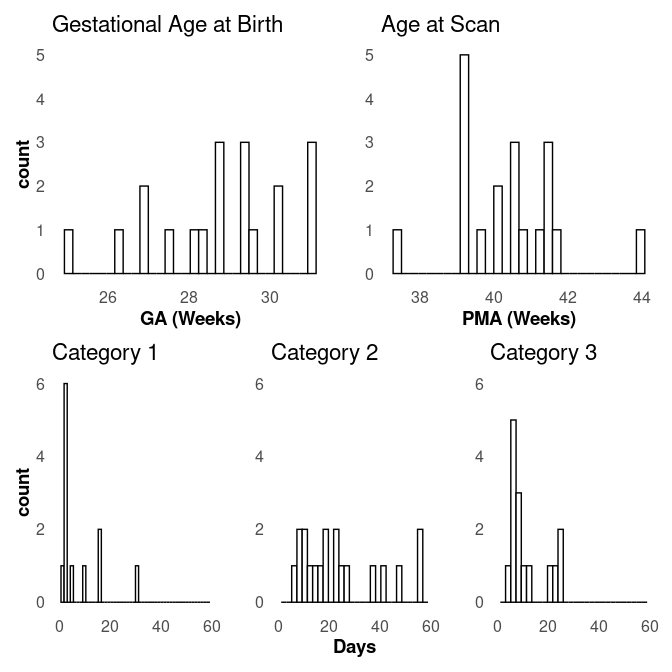
\includegraphics{index_files/figure-latex/notebooks-CMRO2_Analysis-dayscat-output-2.png}

\textsubscript{Source:
\href{https://WeberLab.github.io/CMRO2_Manuscript/notebooks/CMRO2_Analysis.qmd.html\#cell-dayscat}{NatalieCNN}}

}

\caption{\label{fig-dayscat}\textbf{Types of respiratory support in
relation to gestational age at birth, post-menstrual age (PMA) at scan,
and days on each type of respiratory support.} Note, counts of 0 days on
respiratory support are not shown. Category 1 = invasive ventilation;
category 2 = noninvasive ventilation; category 3 = high-flow and
low-flow support.}

\end{figure}%

A subject-by-subject distribution of days on different categories of
respiratory support is shown in Figure~\ref{fig-distribution}.

\begin{figure}

\centering{

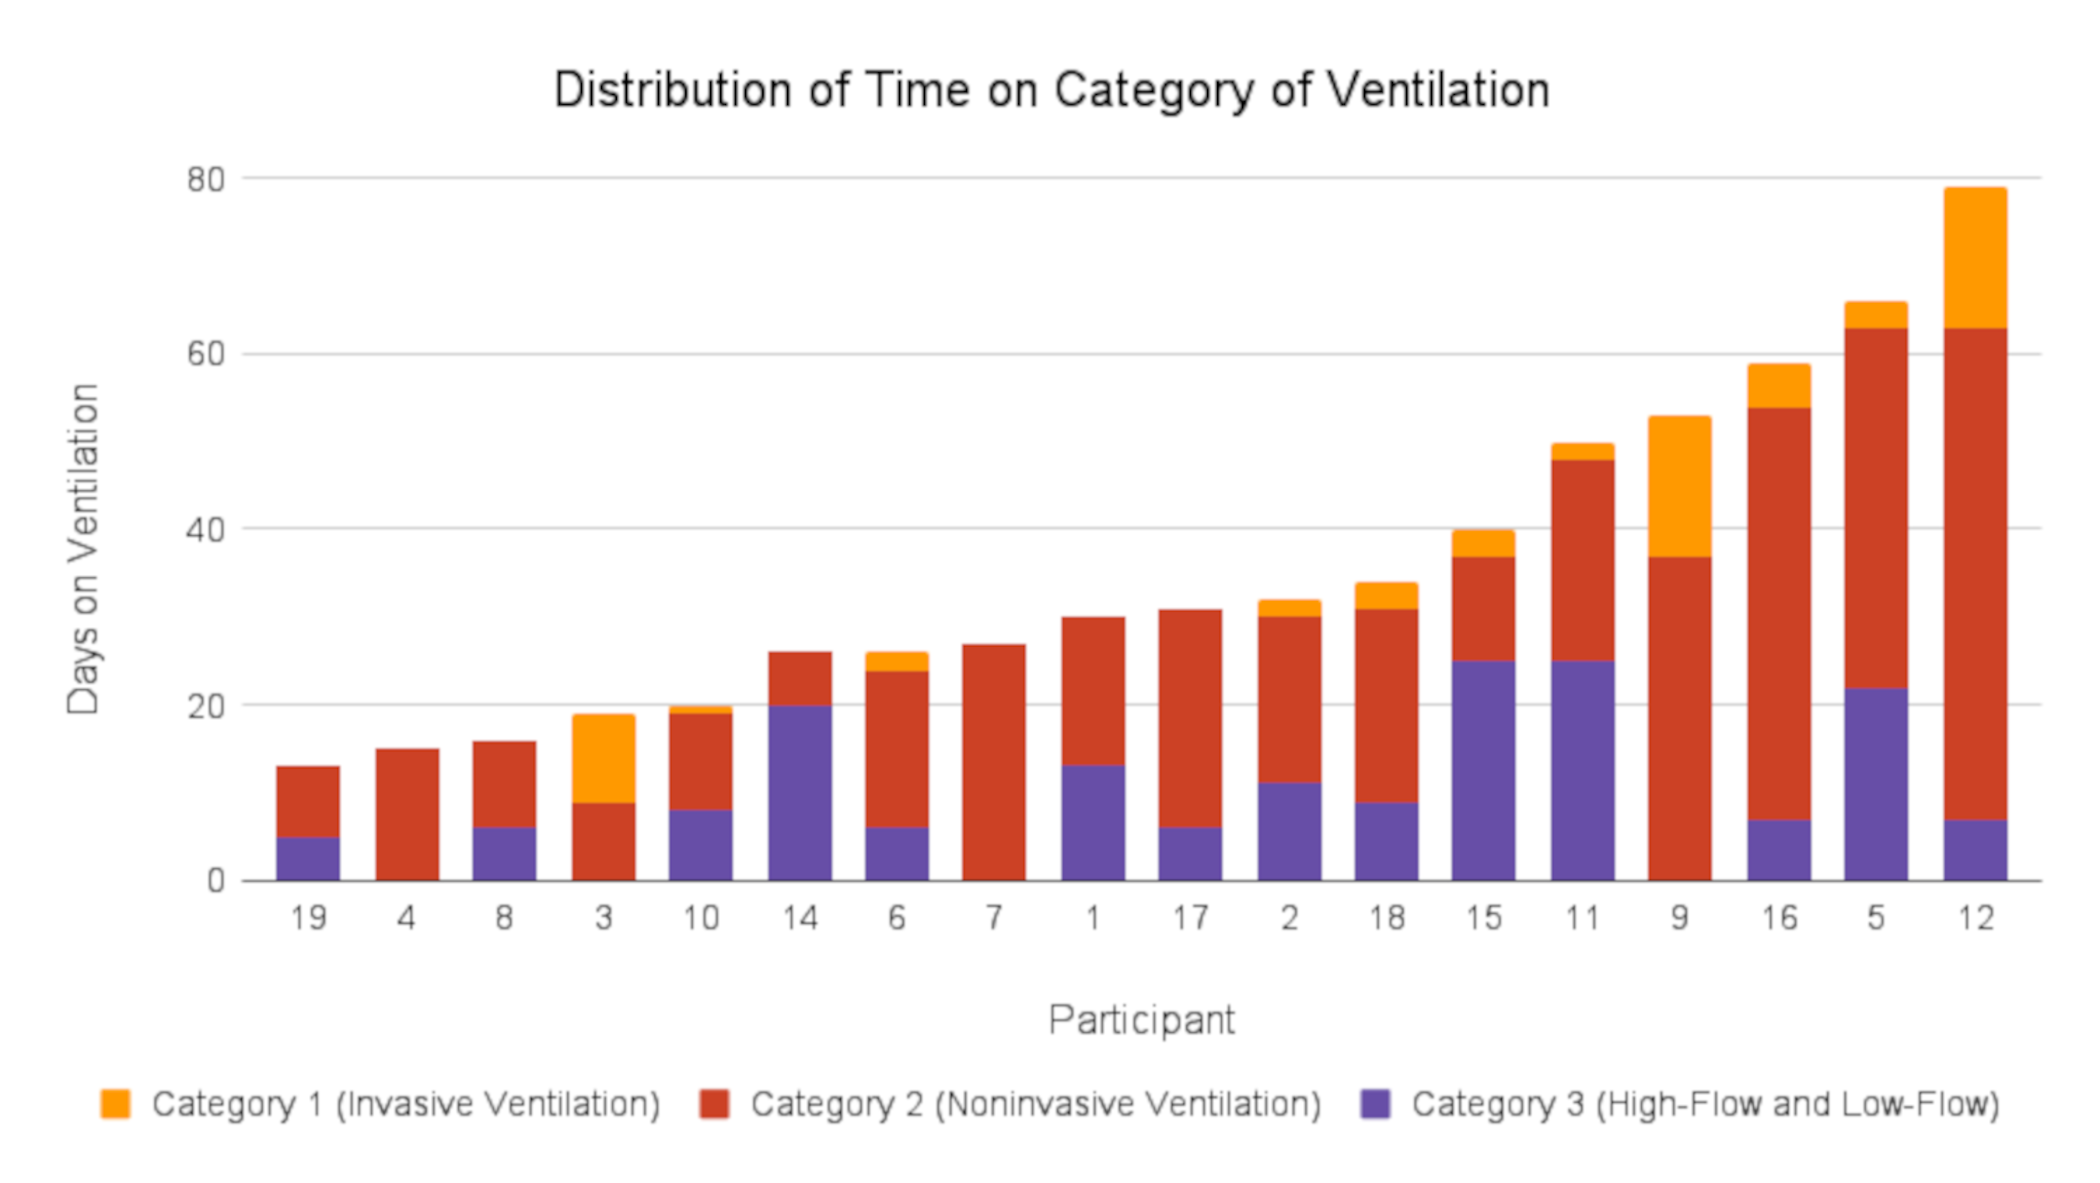
\includegraphics{./Figures/Figure2_Distribution of Time on Category of Ventilation_font.png}

}

\caption{\label{fig-distribution}\textbf{Days on the three levels of
respiratory support for each study subject.}}

\end{figure}%

Gestational age at birth was found to be negatively correlated with both
days on Category 1 (invasive ventilation) and Category 2 (non-invasive
ventilation) respiratory support, but not Category 3
(high-flow/low-flow; Figure~\ref{fig-linreg}).

\begin{figure}

\centering{

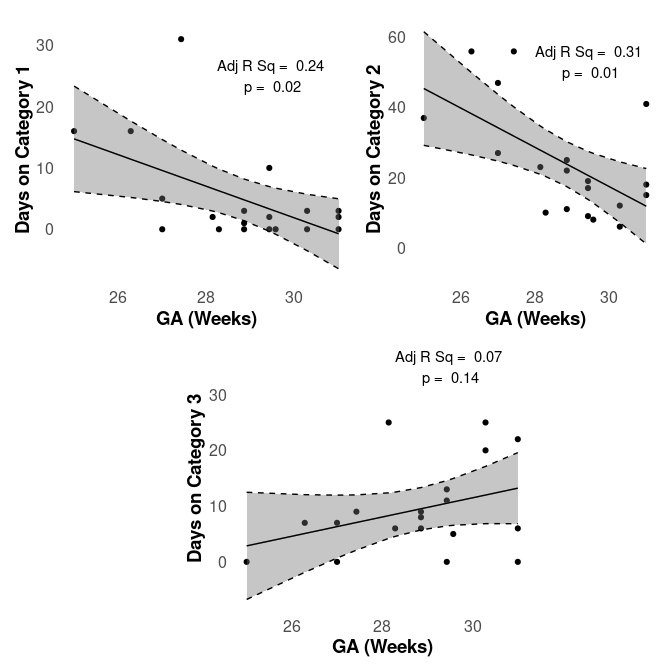
\includegraphics{index_files/figure-latex/.-notebooks-CMRO2_Analysis-linreg-output-2.png}

\textsubscript{Source:
\href{https://WeberLab.github.io/CMRO2_Manuscript/notebooks/CMRO2_Analysis.qmd.html\#cell-linreg}{NatalieCNN}}

}

\caption{\label{fig-linreg}\textbf{Linear regression of days on the
three categories of respiratory support vs gestational age.}}

\end{figure}%

A sample of results of the MRI analysis, including a sample brain
segmentation, CBF map, QSM map, and CMRO\textsubscript{2} map are shown
in Figure~\ref{fig-sampleimages}.

\begin{figure}

\centering{

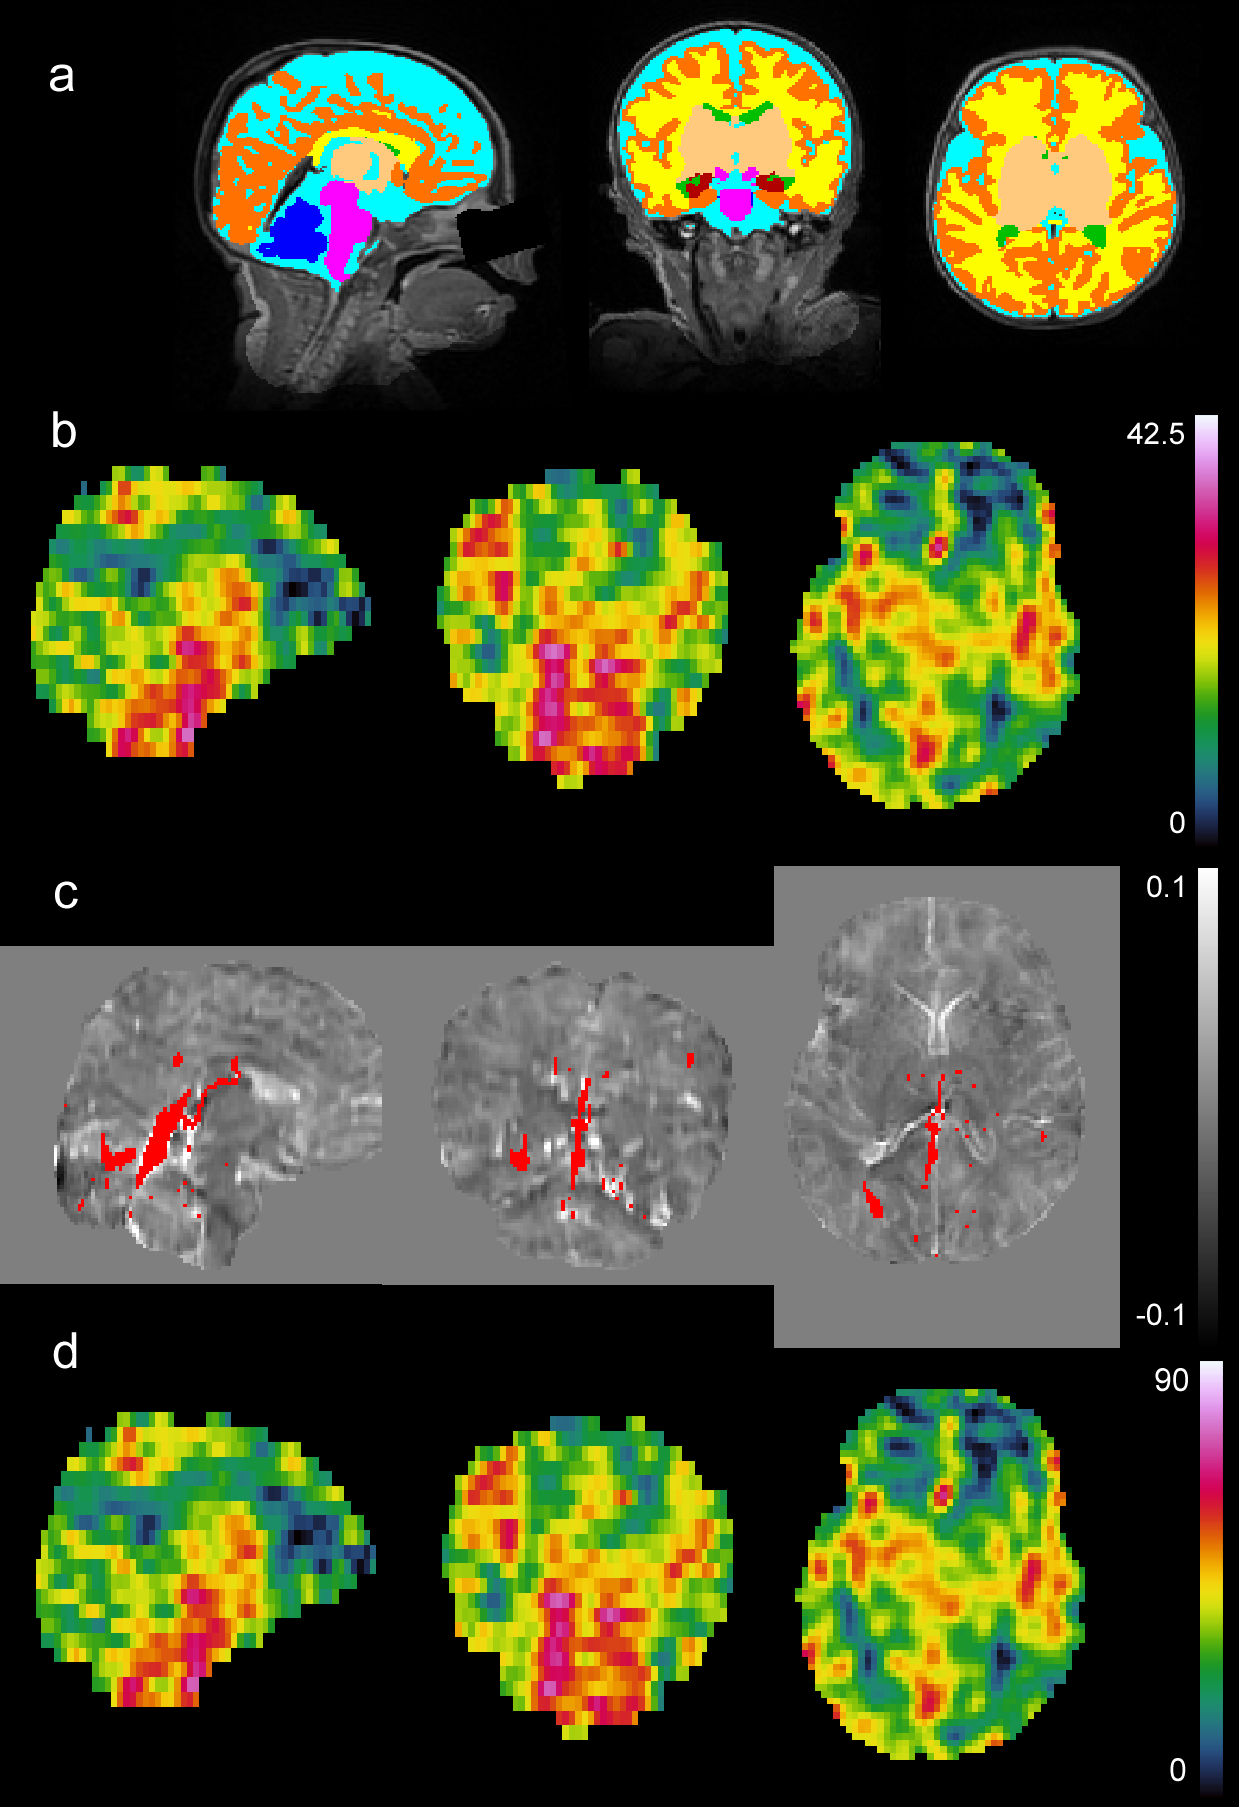
\includegraphics{./Figures/Figure4_combined_300dpi.png}

}

\caption{\label{fig-sampleimages}\textbf{Sample images from a subject of
various MRI results.} All images show a sagittal, coronal and axial
slice from left to right. A) is a T2w image in the background with
segmentation overlaid in various colors: dark blue = cerebellum; pink =
brainstem; light blue = CSF; yellow = white matter; dark orange =
cortical grey matter; green = ventricles; light orange = deep grey
matter; dark red = hippocampus and amygdala. B) is a processed CBF map
from 0 to 47.5 mL/100g/min. C) is a QSM image in the background from
-0.1 to 0.1 ppm susceptibility overlaid with a venous mask in red. D) is
a processed CMRO\textsubscript{2} image from 0 to 93 µmol/100g/min. Note
that B) and D) look identical as D is simply B multiplied by a value
determined by CSaO\textsubscript{2}, CSvO\textsubscript{2}, and Hct.
However, this value will be different for every subject.}

\end{figure}%

Mean whole-brain CSvO\textsubscript{2}, CSaO\textsubscript{2}, Hct and
oxygen extraction fraction (OEF) values were 63.9 ± 4, 98.3 ± 1.5, 29.7
± 3.5, and 34.9 ± 4.3, respectively. Regional mean CBF and
CMRO\textsubscript{2} values are shown in Table~\ref{tbl-regvalues}. The
lowest CBF and CMRO\textsubscript{2} values were found in the WM, while
the highest CBF and CMRO\textsubscript{2} values were found in the
brainstem.

Multiple linear regression analysis of regional CMRO\textsubscript{2}
and CBF showed significant positive correlations with proportion of days
on respiratory support (Figure~\ref{fig-proportion}), days on Category 2
respiratory support (Figure~\ref{fig-cat2}), and significant negative
correlations with days in room air (Figure~\ref{fig-roomair}). Results
are summarized in Table~\ref{tbl-linreg}.

\begin{figure}

\centering{

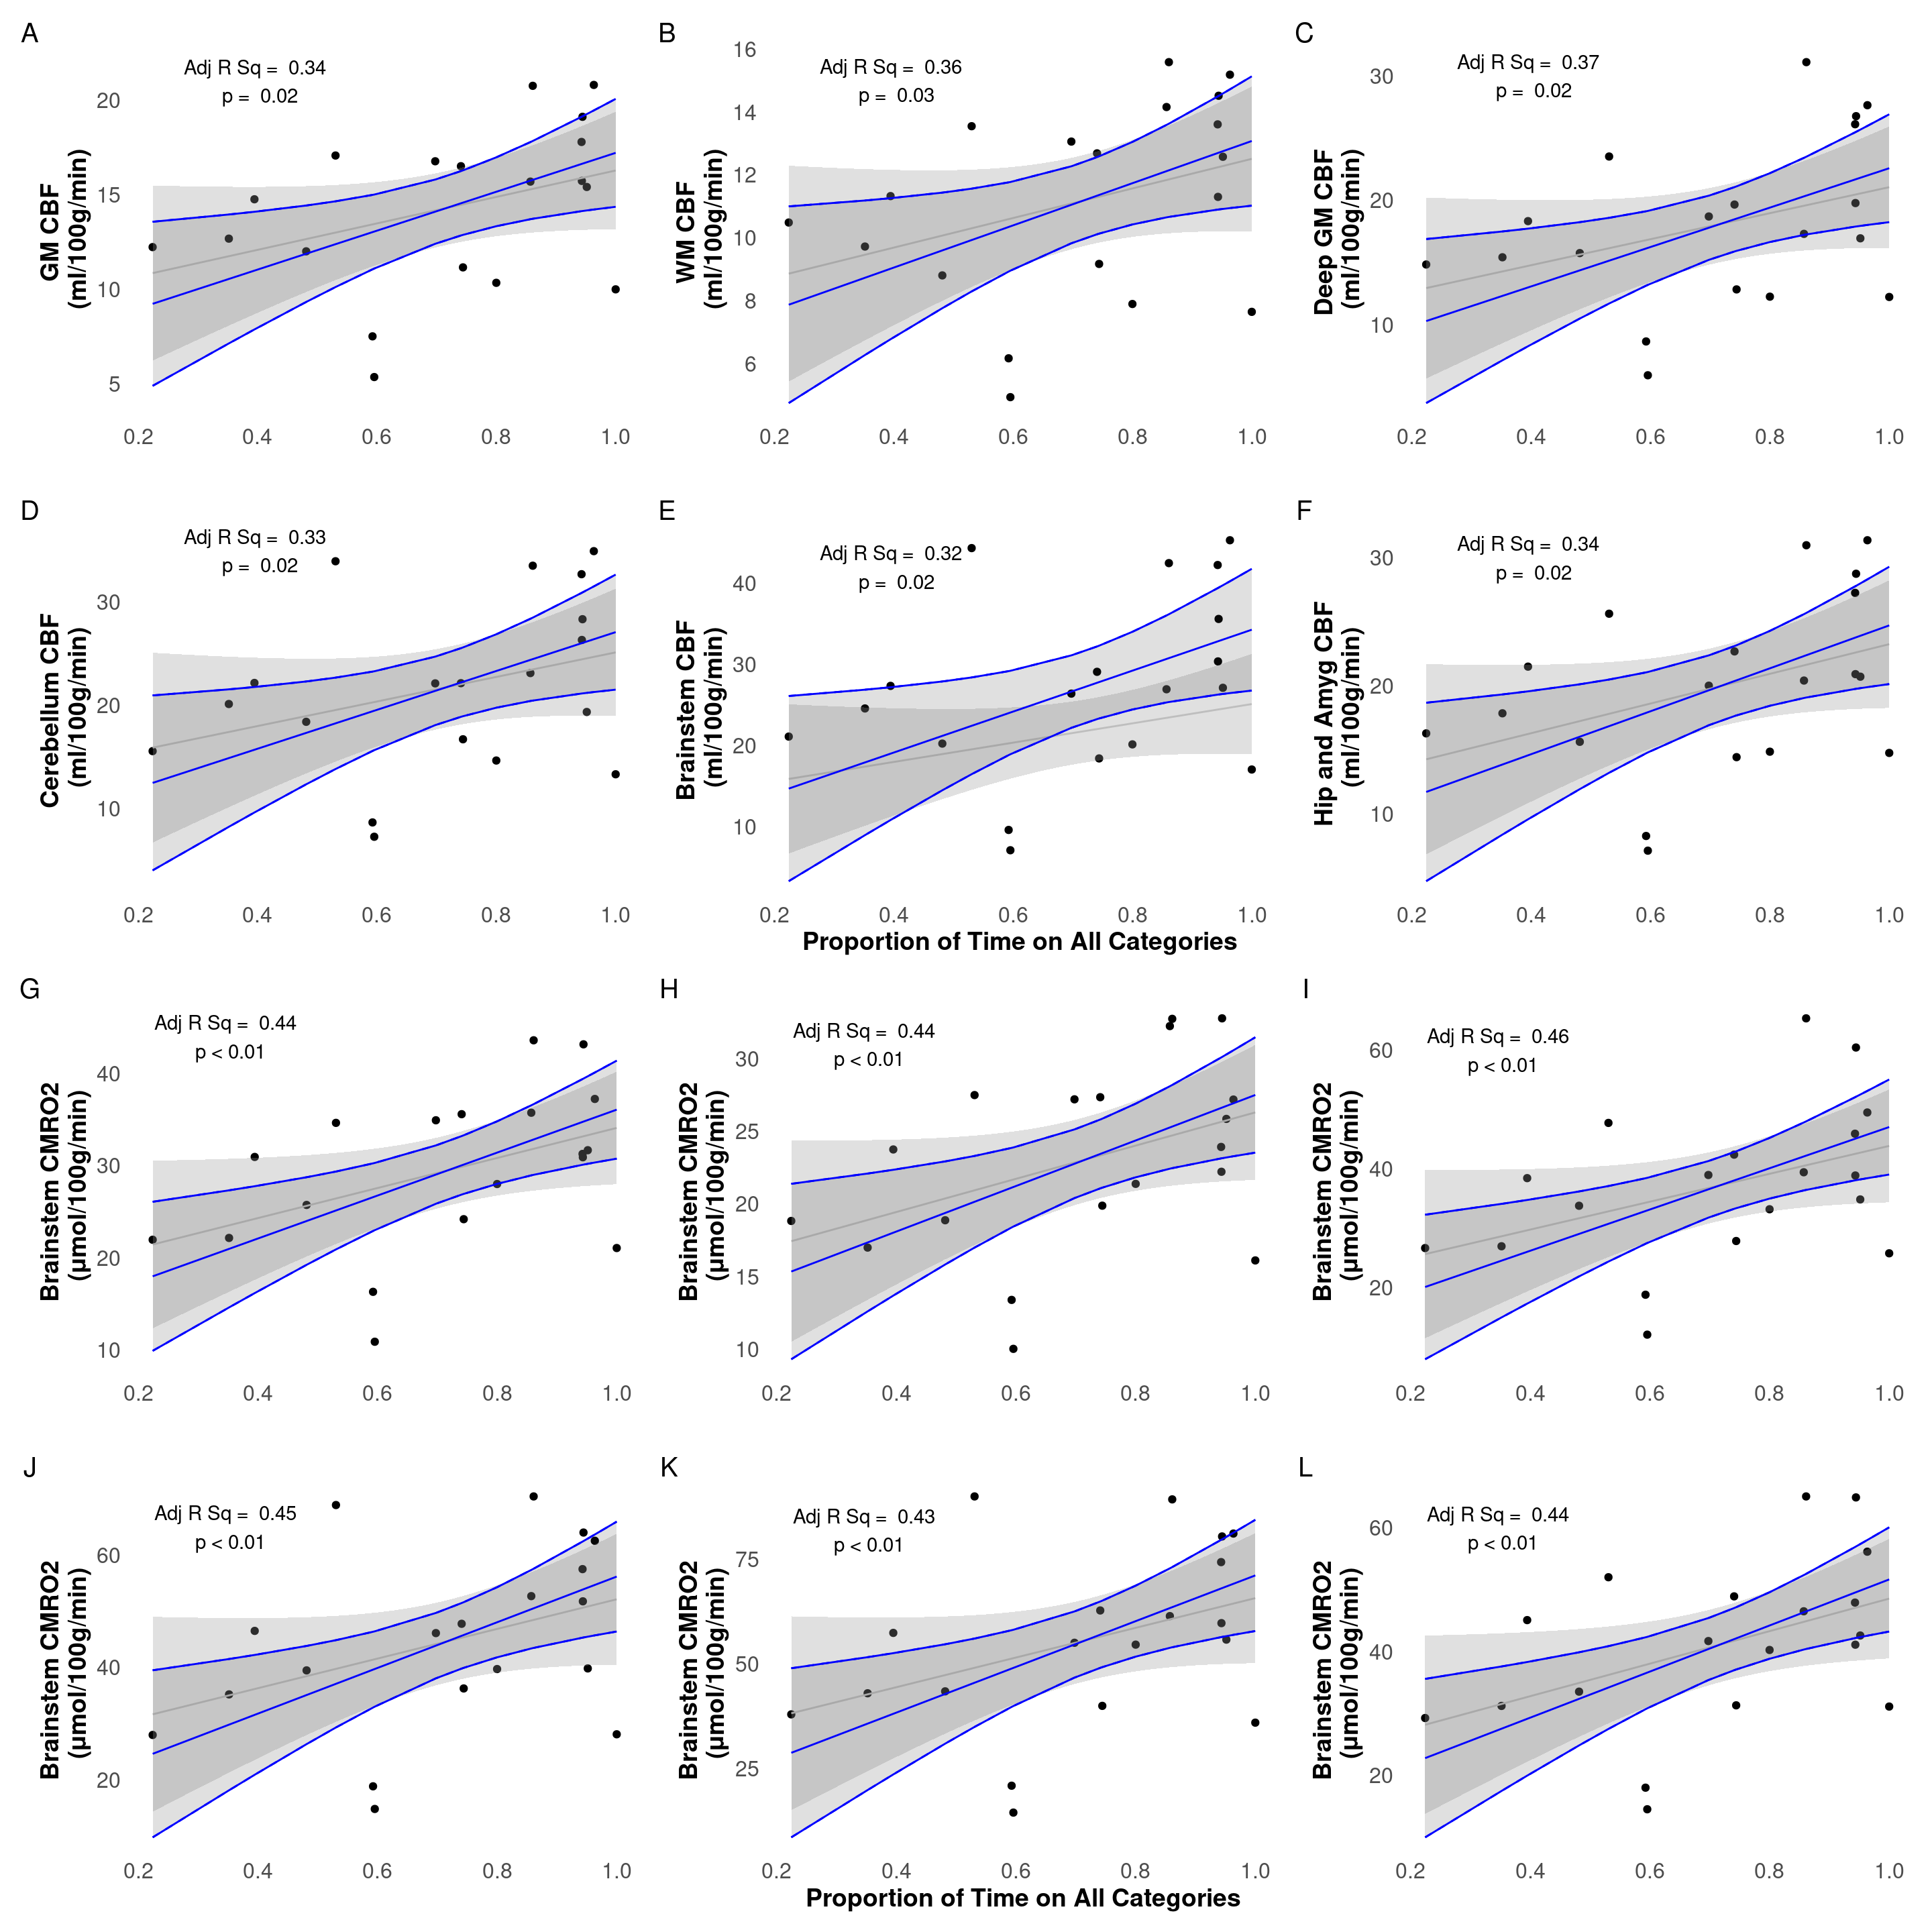
\includegraphics{index_files/figure-latex/.-notebooks-CMRO2_Analysis-proportion-output-2.png}

\textsubscript{Source:
\href{https://WeberLab.github.io/CMRO2_Manuscript/notebooks/CMRO2_Analysis.qmd.html\#cell-proportion}{NatalieCNN}}

}

\caption{\label{fig-proportion}\textbf{CBF (A-F) and
CMRO\textsubscript{2} (G-L) vs proportion of time on all categories
while in the NICU.} Raw data points as filled black circles. Grey line
and ribbon represent linear model of raw data points and 95\% interval,
respectively. Blue line and ribbon represent adjusted multiple linear
regression including GA and PMA as confounding factors.}

\end{figure}%

\begin{figure}

\centering{

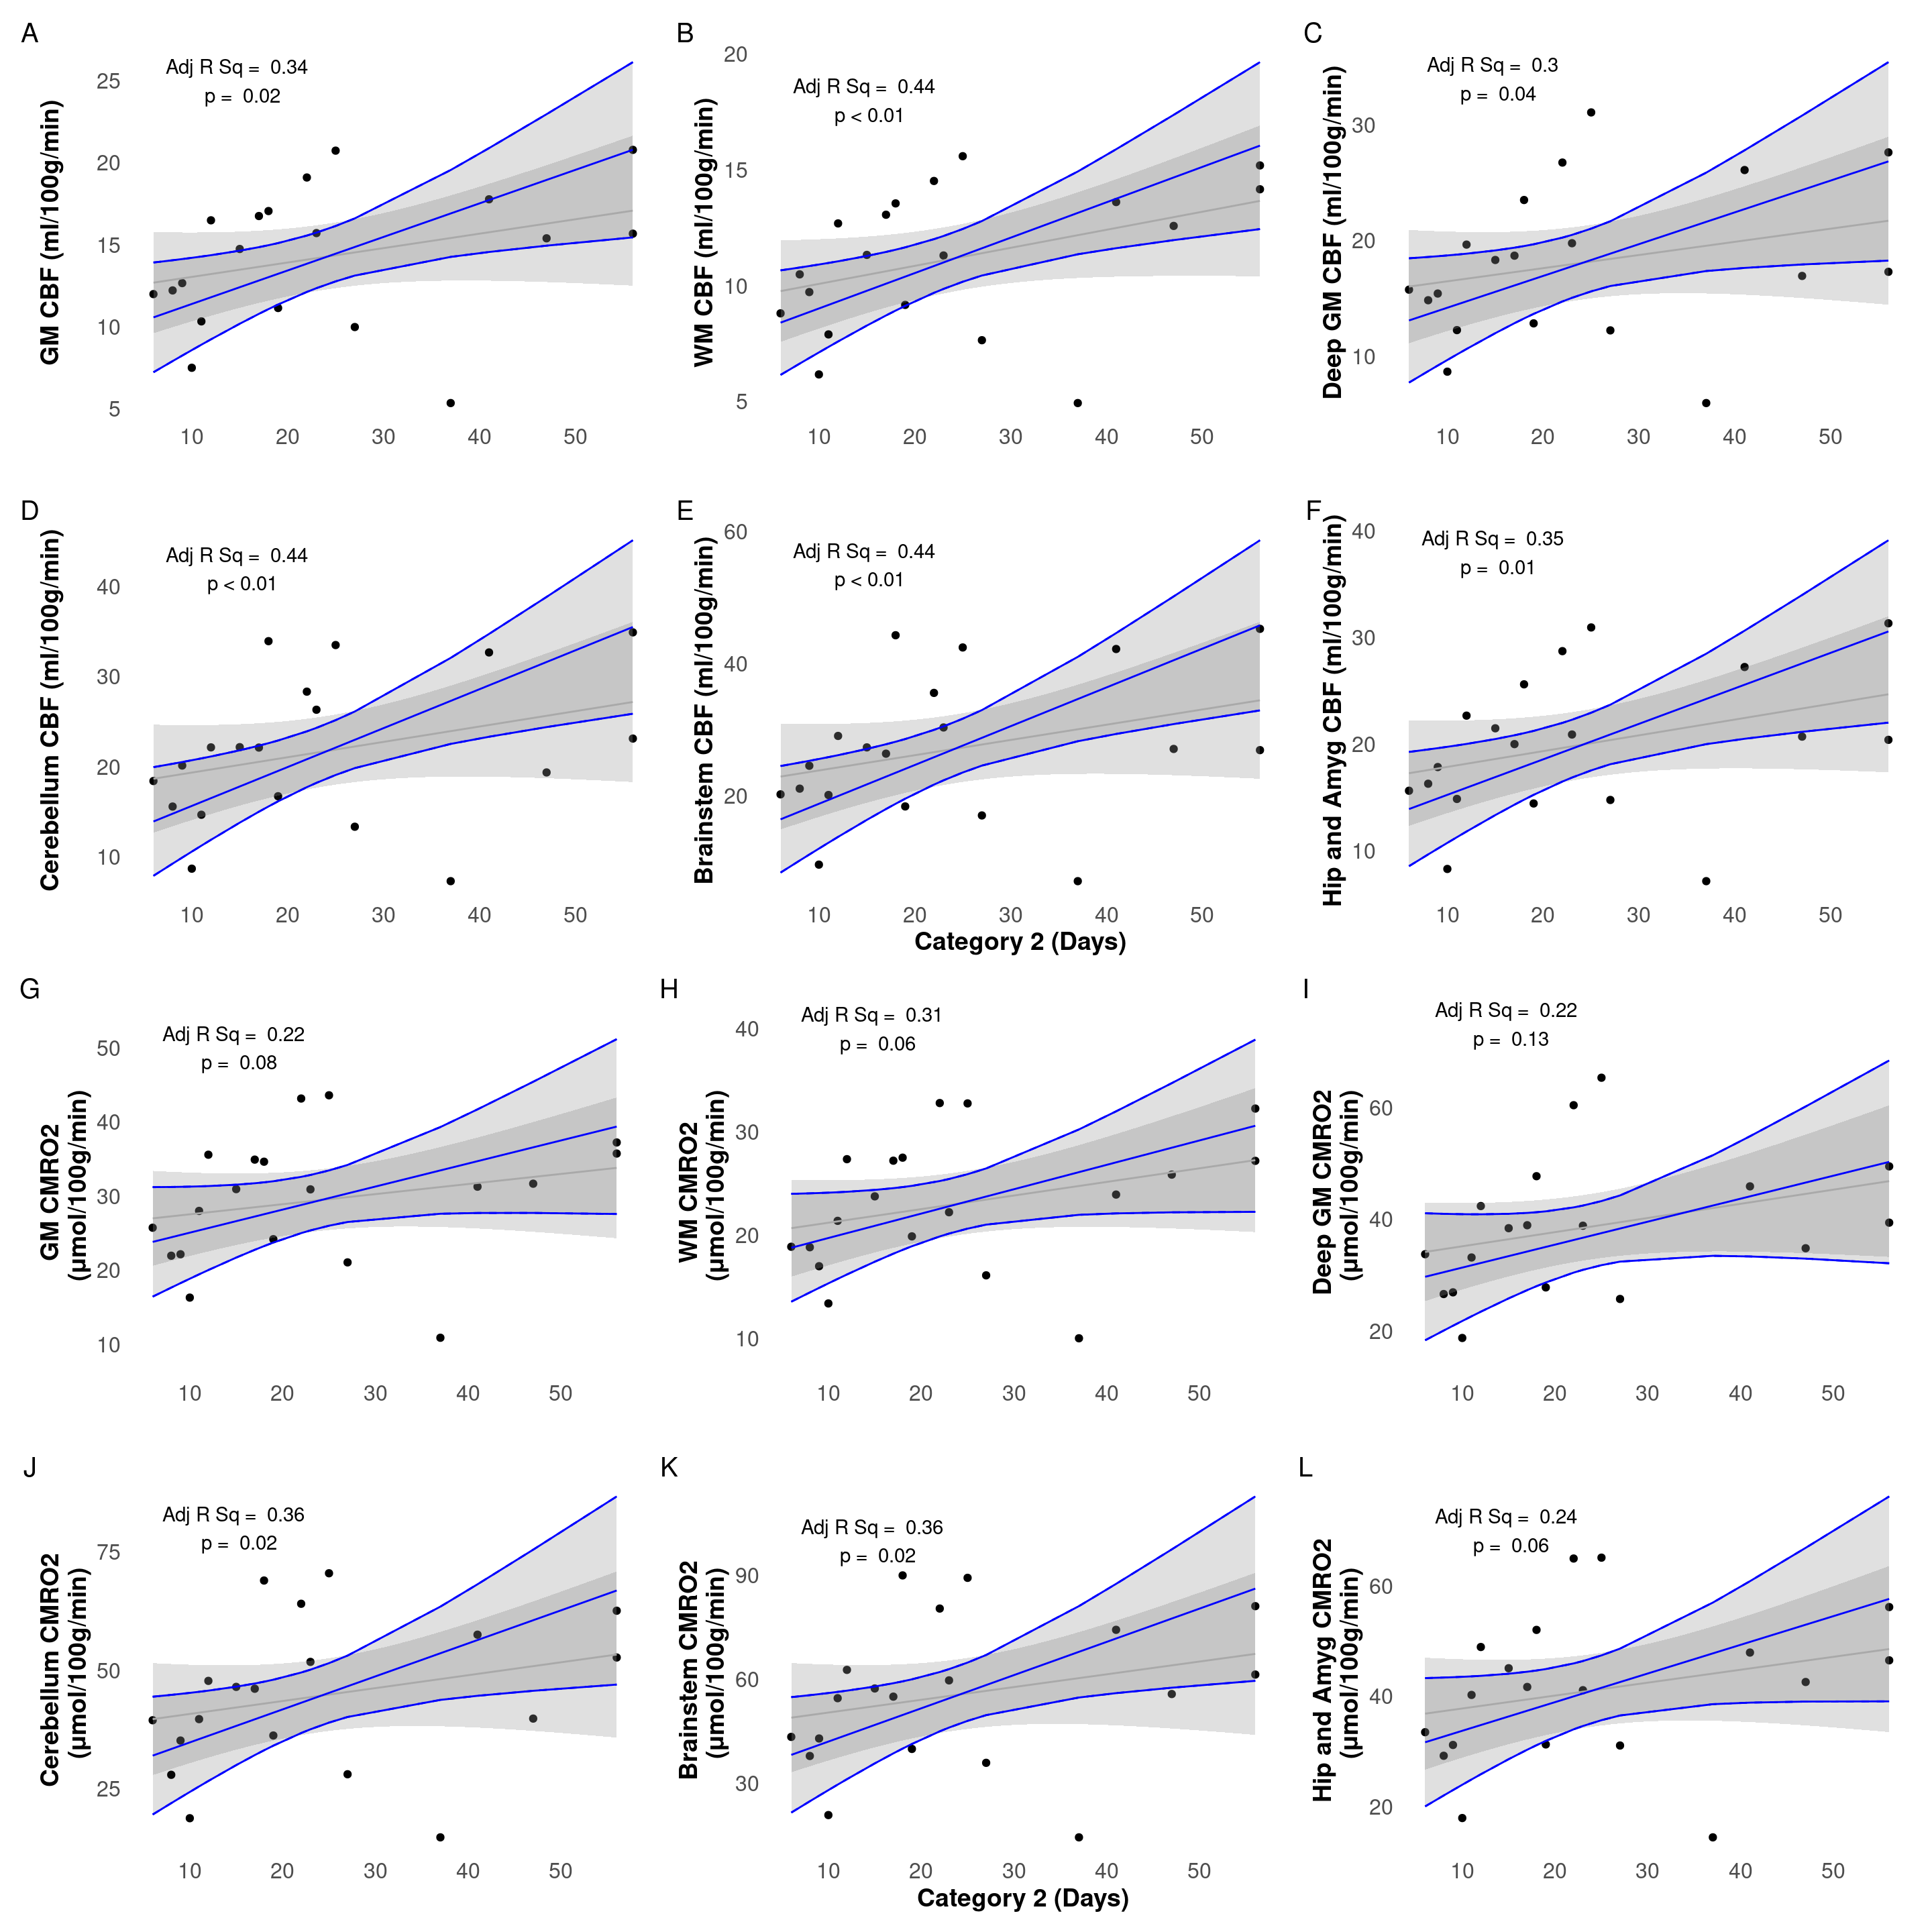
\includegraphics{index_files/figure-latex/.-notebooks-CMRO2_Analysis-cat2-output-2.png}

\textsubscript{Source:
\href{https://WeberLab.github.io/CMRO2_Manuscript/notebooks/CMRO2_Analysis.qmd.html\#cell-cat2}{NatalieCNN}}

}

\caption{\label{fig-cat2}\textbf{CBF (A-F) and CMRO\textsubscript{2}
(G-L) values against Days on Noninvasive Ventilation (Category 2).} Raw
data points as filled black circles. Grey line and ribbon represent
linear model of raw data points and 95\% interval, respectively. Blue
line and ribbon represent adjusted multiple linear regression including
GA and PMA as confounding factors.}

\end{figure}%

\begin{figure}

\centering{

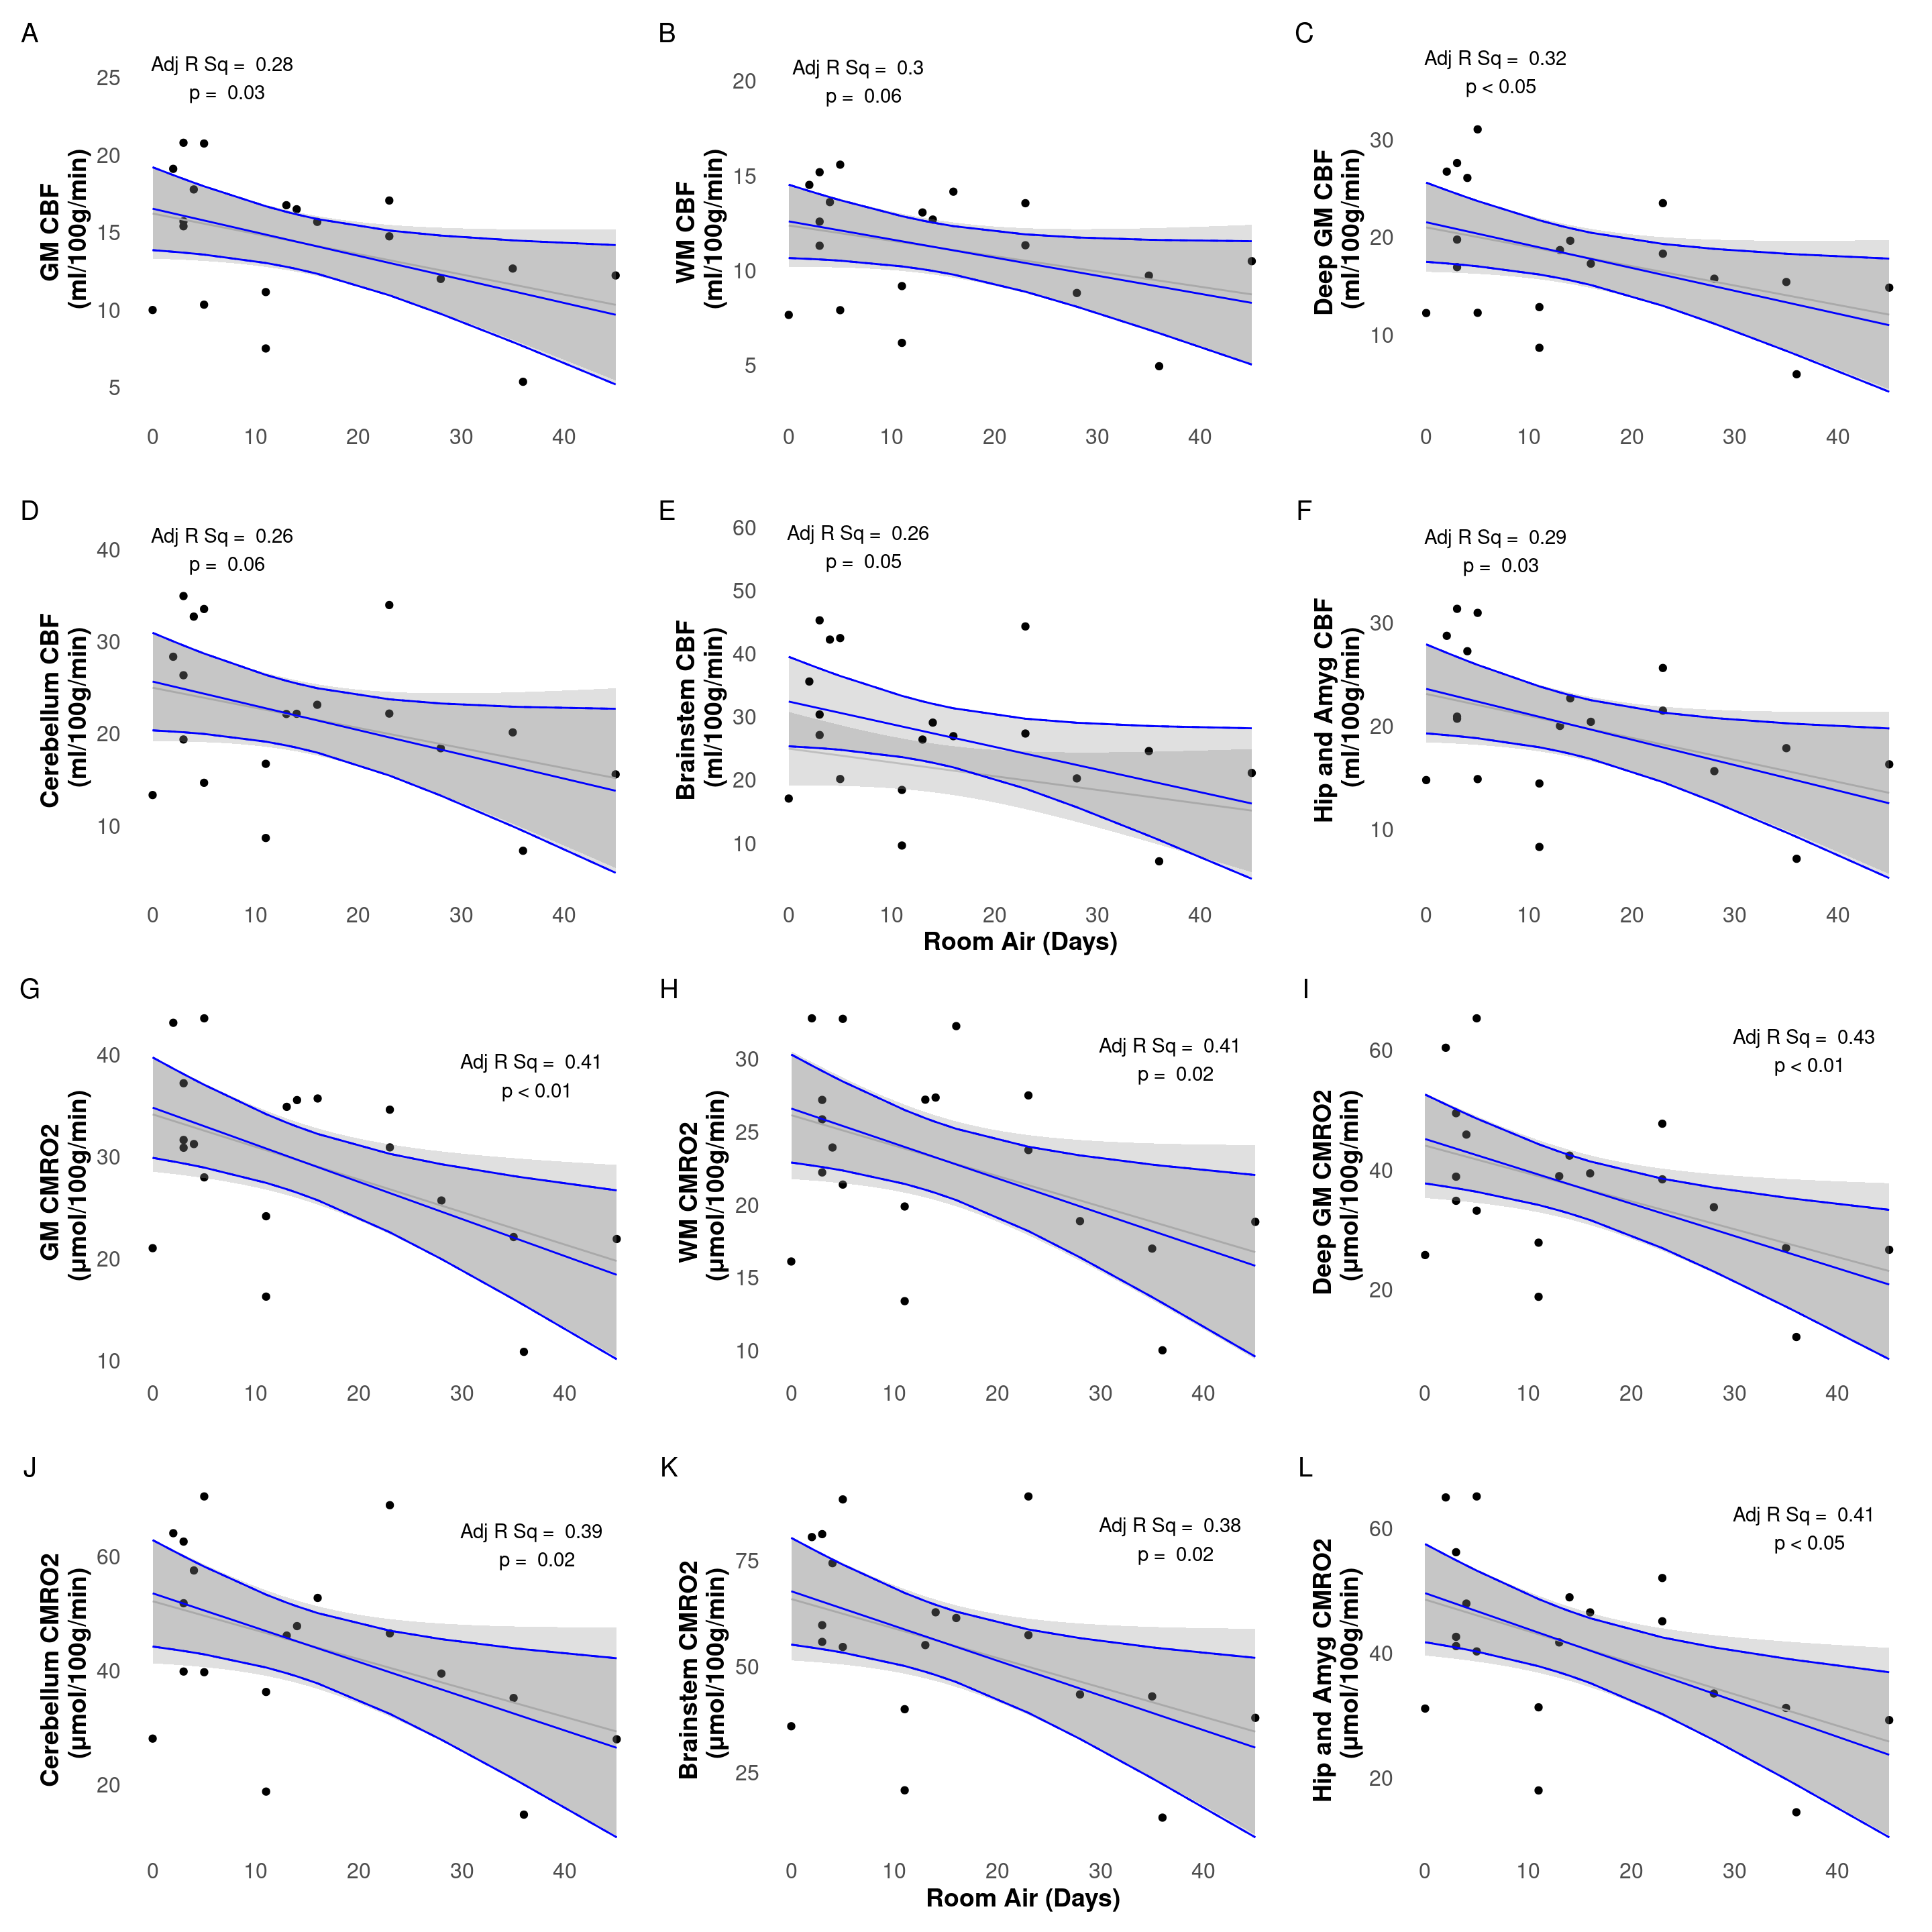
\includegraphics{index_files/figure-latex/.-notebooks-CMRO2_Analysis-roomair-output-2.png}

\textsubscript{Source:
\href{https://WeberLab.github.io/CMRO2_Manuscript/notebooks/CMRO2_Analysis.qmd.html\#cell-roomair}{NatalieCNN}}

}

\caption{\label{fig-roomair}\textbf{CBF () and CMRO\textsubscript{2} (b)
values vs days in room air.} Raw data points as filled black circles.
Grey line and ribbon represent linear model of raw data points and 95\%
interval, respectively. Blue line and ribbon represent adjusted multiple
linear regression including GA and PMA as confounding factors.}

\end{figure}%

No significant relationships were found between respiratory support
categories and OEF, CSvO\textsubscript{2}, CSaO\textsubscript{2}, Hct
(Table~\ref{tbl-linreg}). No significant relationship was observed
between brainstem volume and days on Category 1 respiratory support.

\section{Discussion}\label{discussion}

We presented the initial results of a novel, non-invasive MRI method and
analysis pipeline to evaluate CSvO\textsubscript{2}, OEF and
CMRO\textsubscript{2} in preterm neonates. The values we found agreed
well with earlier reported reference values. In addition, our technique
allowed us to examined the effects of various forms of respiratory
support on CBF and CMRO\textsubscript{2} in neonates born very preterm.
We found that the proportion of days on respiratory support was
positively associated with both CBF and CMRO\textsubscript{2} in all
brain regions, a negative association was found for both CBF (some brain
regions) and CMRO\textsubscript{2} (all brain regions) with days in room
air, and non-invasive ventilation showed a positive association with CBF
in all regions, and a positive association with CMRO\textsubscript{2} in
the brainstem and cerebellum.

\subsection{Comparison of MRI methods with previous
literature}\label{comparison-of-mri-methods-with-previous-literature}

The results from previous neonatal studies are summarized in
Table~\ref{tbl-litvalues}. The global CMRO\textsubscript{2}, CBF, OEF
and CSvO\textsubscript{2} values from this study align well with the
literature from MRI, NIRS and PET studies reported for TEA infants.

One strength of using ASL compared to similar studies that used
phase-contrast to calculate CBF is the ability to look at regional
changes in CBF as opposed to a single number for the whole-brain (Liu et
al. 2014; Qi et al. 2018). This is best demonstrated in the difference
we see when looking at correlations with Category 2, where all regions
were found to have a positive correlation with CBF, but only the
brainstem and cerebellum were found to be positively correlated with
CMRO\textsubscript{2}. This discrepancy is discussed more below.
However, using ASL in infants also has drawbacks that should be
considered, including low signal-to-noise ratio, quantification
difficulties due to uncertainty in labelling efficiency and bolus
arrival time, and the rapid changes that occur in such young populations
that make single-imaging-protocol difficult (Liu et al. 2019).

Similarly, a strength of using QSM to study CSvO\textsubscript{2} rather
than previous MRI methods that used the TRUST (Liu et al. 2014; Qi et
al. 2018) or T2-TRIR (De Vis et al. 2014), is that QSM produces a
whole-brain map with high spatial resolution. By producing a whole-brain
map, we were able to measure the CSvO\textsubscript{2} by averaging over
all internal veins. This is likely to produce a more robust measurement
than acquiring a single slice and averaging within the superior sagittal
sinus (SSS) as TRUST and T2-TRIR do. For the current study, our QSM maps
were reconstructed to a 0.9x0.9x0.9mm\textsuperscript{3} resolution, but
future studies would benefit from acquiring and reconstructing up to
0.5x0.5x0.5 mm\textsubscript{3}. Indeed, greater spatial resolution
would likely improve CSvO\textsubscript{2} measurements as \(\chi\)
values could be better isolated to venous tissue without including
non-venous sources. Finally, QSM could also allow for regional analysis
of CSvO\textsubscript{2} values, which we did not attempt here.
Unfortunately, as our method for calculating QSM requires removing brain
tissue along the edge of the brain (an eroded brain mask), we could not
measure CSvO\textsubscript{2} values in the SSS for more direct
comparisons. Future work should be directed at acquiring QSM values in
the SSS.

Two of the studies that measured CMRO\textsubscript{2}, CBF and
CSvO\textsubscript{2} in sick newborns requiring ventilatory support did
not investigate associations between these values and days on various
forms of respiratory support. Therefore, we were not able to directly
compare these findings.

\subsection{Respiratory support}\label{respiratory-support}

In the present study, more days in room air without any type of
respiratory support was associated with lower CMRO\textsubscript{2} and
CBF values. If the assumption of higher CMRO\textsubscript{2} and CBF
are indications of more optimal brain health, then this may suggest that
the use of some form of respiratory support may be more beneficial to
very preterm infants than weaning to room air. Indeed,
CMRO\textsubscript{2} and CBF were positively related to the proportion
of time on respiratory support compared to the total time in the NICU.
However, caution must be advised when interpreting these findings. Our
study was observational, therefore, we cannot exclude various
confounding factors, such as various levels of illness which would have
dictated the form of respiratory support the infant received. We may be
observing a compensatory effect, wherein infants who were sicker may
have over-compensated for CBF and CMRO\textsubscript{2} to provide
adequate oxygen. This would imply that increased CMRO\textsubscript{2}
and CBF are a reflection of higher illness severity. It is critical for
future studies to further explore this relationship because, if on the
other hand, being in room air indicates suboptimal cerebral oxygenation
and metabolism, it may significantly influence how infants in the NICU
are managed.

Furthermore, while all brain regions were found to have a negative
correlation between days in room air and CMRO\textsubscript{2}, this was
not the case for CBF, where only the cortical grey matter, deep grey
matter, and hippocampus \& amygdala were found to be negatively
correlated with days in room air. Specific brain structures appear to
regulate the level of CBF differently and independently of
CMRO\textsubscript{2}, suggesting that these brain regions may be more
susceptible to or protected from hypoxia. Indeed, evidence for
physiological uncoupling of CBF and CMRO\textsubscript{2} has been
reported previously (Fox and Raichle 1986; Henriksen et al. 2021; Ishii
et al. 1996). However, caution should be exercised when drawing strong
conclusions from our exploratory analysis.

Invasive ventilation was not found to have to be associated with
CMRO\textsubscript{2} or CBF in any tissue regions. This was unexpected
as we hypothesized that infants who required more days on invasive
ventilatory support would have lower CMRO\textsubscript{2} values at
TEA. We also did not find a relationship between invasive mechanical
ventilation and brain stem volume at TEA, unlike a previous study by
Guillot et al.~(2020) (Guillot et al. 2020). Our results are likely
limited by the low exposure of this population to invasive mechanical
ventilation, as only one infant required invasive support for a
prolonged period of time (\textgreater{} 28days).

Non-invasive ventilation support was associated with increased
CMRO\textsubscript{2} and CBF in preterm neonates at TEA. The observed
increase in CMRO\textsubscript{2} and CBF with non-invasive ventilation
\emph{suggests} that prioritizing non-invasive over invasive ventilation
may improve brain health outcomes in preterm neonates. However, caution
should be exercised as our findings are exploratory in nature. Future
studies on respiratory support strategies should incorporate
CMRO\textsubscript{2} and CBF measurements to better understand their
relationship with cerebral oxygenation and include a healthy term
control cohort to establish comparative baseline values.

The difference between elevated CMRO\textsubscript{2} and CBF was also
observed within regional tissues where CBF increased in all regional
tissues for infants on non-invasive ventilation, but
CMRO\textsubscript{2} only increased in the brainstem and cerebellar
tissue. One possibility for this observation could be that compensatory
mechanisms are activated in response to respiratory distress or regional
brain injuries that hinder the uptake of oxygen. As with our findings in
room air, this suggests that specific brain regions respond to
respiratory support differently and may be more susceptible to damage.
However, further research is first required to reproduce our exploratory
findings.

\subsection{Limitations}\label{limitations}

There are several limitations that are worth highlighting. Our
CSvO\textsubscript{2} processing pipeline filtered out \(\chi\) values
below 0.15 ppm in order to obtain realistic values. Future studies may
wish to use smaller voxel sizes, as well as a technique to decompose
paramagnetic and diamagnetic values in order to avoid this step (Shin et
al. 2021). See a recent study of ours for an attempt at this technique
(Carmichael et al. 2025). Furthermore, in order to reduce QSM artifacts,
the exterior of the brain mask was eroded, making it impossible to
measure CSvO\textsubscript{2} in the SSS. Future studies may find a way
to measure QSM in the SSS, which would also allow researchers to
determine if CSvO\textsubscript{2} values are different in the SSS
compared to the central cerebral veins. Again, see a recent study of
ours that attempted this (Carmichael et al. 2025). Hct levels were not
collected on the day of the scan, but instead were predicted based on
past values. Our respiratory support analysis was exploratory with a
small sample size. Thus, the positive correlation we found in Category 2
may be spurious or a result of an unaccounted factor. Future studies
using large sample randomized controlled trials would provide a clearer
understanding of the relationship between respiratory support and
cerebral oxygenation. Imaging was performed at term-equivalent age after
the infants had been discharged from the NICU, meaning the scans were
performed weeks after the infants were last on respiratory support.
Obtaining scans while the infants are still receiving respiratory
support could provide a more robust mechanistic connection. Our study
did not include a healthy control cohort to compare the expected
physiological measures at TEA. This would be important to include, as
too much oxygen can be just as harmful as not enough (Rantakari et al.
2021). Finally, due to our sample size, this study did not explore
supplementary variables, such as medications, that may affect
respiratory uptake and oxygen metabolism, and patterns of oxygen
saturations infants experience during their NICU stay.

\section{Acknowledgments}\label{acknowledgments}

We wish to acknowledge the work of and thank *** (Research Nurse); ***
(Research Nurse); *** (Neonatologist); and *** (Radiologist).

\section{Funding}\label{funding}

Authors *** were co-primary investigators on a *** Catalyst Grant
(\$20,000). *** were supported by an establishment award from *** .
Scanning was partly funded through a special award to *** from *** .

\newpage{}

\section{References}\label{references}

\phantomsection\label{refs}
\begin{CSLReferences}{1}{0}
\bibitem[\citeproctext]{ref-ackermannHighfrequencyVentilationPreterm2023}
Ackermann, Benjamin W., Daniel Klotz, Roland Hentschel, Ulrich H. Thome,
and Anton H. Van Kaam. 2023. {``High-Frequency Ventilation in Preterm
Infants and Neonates.''} \emph{Pediatric Research} 93 (7): 1810--18.
\url{https://doi.org/10.1038/s41390-021-01639-8}.

\bibitem[\citeproctext]{ref-altmanCerebralOxygenMetabolism1993}
Altman, D. I., J. M. Perlman, J. J. Volpe, and W. J. Powers. 1993.
{``\href{https://www.ncbi.nlm.nih.gov/pubmed/8516092}{Cerebral Oxygen
Metabolism in Newborns}.''} \emph{Pediatrics} 92 (1): 99--104.

\bibitem[\citeproctext]{ref-brownMechanicalVentilationPremature2011}
Brown, Melissa K, and Robert M DiBlasi. 2011. {``Mechanical
{Ventilation} of the {Premature Neonate}.''} \emph{Respiratory Care} 56
(9): 1298--1313. \url{https://doi.org/10.4187/respcare.01429}.

\bibitem[\citeproctext]{ref-cannavoVentilationOxidativeStress2020}
Cannavò, Laura, Immacolata Rulli, Raffaele Falsaperla, Giovanni
Corsello, and Eloisa Gitto. 2020. {``Ventilation, Oxidative Stress and
Risk of Brain Injury in Preterm Newborn.''} \emph{Italian Journal of
Pediatrics} 46 (1): 100.
\url{https://doi.org/10.1186/s13052-020-00852-1}.

\bibitem[\citeproctext]{ref-carmichael-etal-magnetic}
Carmichael, Thomas Gavin, Alexander Rauscher, Ruth E. Grunau, and
Alexander Mark Weber. 2025. {``The Application of Magnetic
Susceptibility Separation for Measuring Cerebral Oxygenation in Preterm
Neonates.''} \emph{Pediatric Research}, March.
\url{https://doi.org/10.1038/s41390-025-03966-6}.

\bibitem[\citeproctext]{ref-chungNeurodevelopmentalOutcomesPreterm2020}
Chung, Estefani Hee, Jesse Chou, and Kelly A. Brown. 2020.
{``Neurodevelopmental Outcomes of Preterm Infants: A Recent Literature
Review.''} \emph{Translational Pediatrics} 9 (S1): S3--8.
\url{https://doi.org/10.21037/tp.2019.09.10}.

\bibitem[\citeproctext]{ref-devisNoninvasiveMRIMeasurements2014}
De Vis, J. B., E. T. Petersen, T. Alderliesten, F. Groenendaal, L. S. de
Vries, F. van Bel, M. J. N. L. Benders, and J. Hendrikse. 2014.
{``Non-Invasive {MRI} Measurements of Venous Oxygenation, Oxygen
Extraction Fraction and Oxygen Consumption in Neonates.''}
\emph{NeuroImage} 95 (July): 185--92.
\url{https://doi.org/10.1016/j.neuroimage.2014.03.060}.

\bibitem[\citeproctext]{ref-dhillonCerebralOxygenationMetabolism2022}
Dhillon, Simerdeep K., Eleanor R. Gunn, Benjamin A. Lear, Victoria J.
King, Christopher A. Lear, Guido Wassink, Joanne O. Davidson, Laura
Bennet, and Alistair J. Gunn. 2022. {``Cerebral {Oxygenation} and
{Metabolism After Hypoxia-Ischemia}.''} \emph{Frontiers in Pediatrics}
10 (July): 925951. \url{https://doi.org/10.3389/fped.2022.925951}.

\bibitem[\citeproctext]{ref-dumpaNonInvasiveVentilatoryStrategies2021}
Dumpa, Vikramaditya, and Vineet Bhandari. 2021. {``Non-{Invasive
Ventilatory Strategies} to {Decrease Bronchopulmonary
Dysplasia}---{Where Are We} in 2021?''} \emph{Children} 8 (2): 132.
\url{https://doi.org/10.3390/children8020132}.

\bibitem[\citeproctext]{ref-elwellMeasurementCMRO2Neonates2005}
Elwell, Clare E., Julian R. Henty, Terence S. Leung, Topun Austin,
Judith H. Meek, David T. Delpy, and John S. Wyatt. 2005. {``Measurement
of {CMRO2} in {Neonates Undergoing Intensive Care Using Near Infrared
Spectroscopy}.''} In \emph{Oxygen {Transport} to {Tissue XXVI}}, edited
by Paul Okunieff, Jacqueline Williams, and Yuhchyau Chen, 566:263--68.
New York: Springer-Verlag.
\url{https://doi.org/10.1007/0-387-26206-7_35}.

\bibitem[\citeproctext]{ref-foxFocalPhysiologicalUncoupling1986}
Fox, P T, and M E Raichle. 1986. {``Focal Physiological Uncoupling of
Cerebral Blood Flow and Oxidative Metabolism During Somatosensory
Stimulation in Human Subjects.''} \emph{Proceedings of the National
Academy of Sciences} 83 (4): 1140--44.
\url{https://doi.org/10.1073/pnas.83.4.1140}.

\bibitem[\citeproctext]{ref-greenoughOptimalStrategiesNewborn2005}
Greenough, Anne, and Atul Sharma. 2005. {``Optimal Strategies for
Newborn Ventilation---a Synthesis of the Evidence.''} \emph{Early Human
Development} 81 (12): 957--64.
\url{https://doi.org/10.1016/j.earlhumdev.2005.10.002}.

\bibitem[\citeproctext]{ref-guillotMechanicalVentilationDuration2020}
Guillot, Mireille, Ting Guo, Steven Ufkes, Juliane Schneider, Anne
Synnes, Vann Chau, Ruth E. Grunau, and Steven P. Miller. 2020.
{``Mechanical {Ventilation Duration}, {Brainstem Development}, and
{Neurodevelopment} in {Children Born Preterm}: {A Prospective Cohort
Study}.''} \emph{The Journal of Pediatrics} 226 (November): 87--95.e3.
\url{https://doi.org/10.1016/j.jpeds.2020.05.039}.

\bibitem[\citeproctext]{ref-henriksenRegionalInterindividualRelationships2021}
Henriksen, Otto M., Albert Gjedde, Kim Vang, Ian Law, Joel Aanerud, and
Egill Rostrup. 2021. {``Regional and Interindividual Relationships
Between Cerebral Perfusion and Oxygen Metabolism.''} \emph{Journal of
Applied Physiology} 130 (6): 1836--47.
\url{https://doi.org/10.1152/japplphysiol.00939.2020}.

\bibitem[\citeproctext]{ref-hoContinuousPositiveAirway2020}
Ho, Jacqueline J, Prema Subramaniam, and Peter G Davis. 2020.
{``Continuous Positive Airway Pressure ({CPAP}) for Respiratory Distress
in Preterm Infants.''} Edited by Cochrane Neonatal Group. \emph{Cochrane
Database of Systematic Reviews} 2020 (10).
\url{https://doi.org/10.1002/14651858.CD002271.pub3}.

\bibitem[\citeproctext]{ref-ishiiRegionalDifferenceCerebral1996}
Ishii, K., M. Sasaki, H. Kitagaki, S. Sakamoto, S. Yamaji, and K. Maeda.
1996. {``\href{https://www.ncbi.nlm.nih.gov/pubmed/8965174}{Regional
Difference in Cerebral Blood Flow and Oxidative Metabolism in Human
Cortex}.''} \emph{Journal of Nuclear Medicine: Official Publication,
Society of Nuclear Medicine} 37 (7): 1086--88.

\bibitem[\citeproctext]{ref-jainCerebralOxygenMetabolism2014}
Jain, Varsha, Erin M. Buckley, Daniel J. Licht, Jennifer M. Lynch, Peter
J. Schwab, Maryam Y. Naim, Natasha A. Lavin, et al. 2014. {``Cerebral
Oxygen Metabolism in Neonates with Congenital Heart Disease Quantified
by {MRI} and Optics.''} \emph{Journal of Cerebral Blood Flow and
Metabolism: Official Journal of the International Society of Cerebral
Blood Flow and Metabolism} 34 (3): 380--88.
\url{https://doi.org/10.1038/jcbfm.2013.214}.

\bibitem[\citeproctext]{ref-jainRapidMagneticResonance2011}
Jain, Varsha, Michael C Langham, Thomas F Floyd, Gaurav Jain, Jeremy F
Magland, and Felix W Wehrli. 2011. {``Rapid Magnetic Resonance
Measurement of Global Cerebral Metabolic Rate of Oxygen Consumption in
Humans During Rest and Hypercapnia.''} \emph{Journal of Cerebral Blood
Flow \& Metabolism} 31 (7): 1504--12.
\url{https://doi.org/10.1038/jcbfm.2011.34}.

\bibitem[\citeproctext]{ref-kalikkotthekkeveeduVentilationInducedLungInjury2022}
Kalikkot Thekkeveedu, Renjithkumar, Ahmed El-Saie, Varsha Prakash,
Lakshmi Katakam, and Binoy Shivanna. 2022. {``Ventilation-{Induced Lung
Injury} ({VILI}) in {Neonates}: {Evidence-Based Concepts} and
{Lung-Protective Strategies}.''} \emph{Journal of Clinical Medicine} 11
(3): 557. \url{https://doi.org/10.3390/jcm11030557}.

\bibitem[\citeproctext]{ref-kiechl-kohlendorferAdverseNeurodevelopmentalOutcome2009}
Kiechl-Kohlendorfer, U, E Ralser, U Pupp Peglow, G Reiter, and R
Trawöger. 2009. {``Adverse Neurodevelopmental Outcome in Preterm
Infants: Risk Factor Profiles for Different Gestational Ages.''}
\emph{Acta Paediatrica} 98 (5): 792--96.
\url{https://doi.org/10.1111/j.1651-2227.2009.01219.x}.

\bibitem[\citeproctext]{ref-kollisch-singuleMechanicalVentilationPediatric2022}
Kollisch-Singule, Michaela, Harry Ramcharran, Joshua Satalin, Sarah
Blair, Louis A. Gatto, Penny L. Andrews, Nader M. Habashi, Gary F.
Nieman, and Adel Bougatef. 2022. {``Mechanical {Ventilation} in
{Pediatric} and {Neonatal Patients}.''} \emph{Frontiers in Physiology}
12 (March): 805620. \url{https://doi.org/10.3389/fphys.2021.805620}.

\bibitem[\citeproctext]{ref-liuQuantitativeAssessmentGlobal2014}
Liu, Peiying, Hao Huang, Nancy Rollins, Lina F. Chalak, Tina Jeon, Cathy
Halovanic, and Hanzhang Lu. 2014. {``Quantitative Assessment of Global
Cerebral Metabolic Rate of Oxygen ({CMRO2}) in Neonates Using {MRI}.''}
\emph{NMR in Biomedicine} 27 (3): 332--40.
\url{https://doi.org/10.1002/nbm.3067}.

\bibitem[\citeproctext]{ref-liuAssessmentCerebralBlood2019}
Liu, Peiying, Ying Qi, Zixuan Lin, Qiyong Guo, Xiaoming Wang, and
Hanzhang Lu. 2019. {``Assessment of Cerebral Blood Flow in Neonates and
Infants: {A} Phase-Contrast {MRI} Study.''} \emph{NeuroImage} 185
(January): 926--33.
\url{https://doi.org/10.1016/j.neuroimage.2018.03.020}.

\bibitem[\citeproctext]{ref-luQuantitativeEvaluationOxygenation2008}
Lu, Hanzhang, and Yulin Ge. 2008. {``Quantitative Evaluation of
Oxygenation in Venous Vessels Using {T2-Relaxation-Under-Spin-Tagging
MRI}.''} \emph{Magnetic Resonance in Medicine} 60 (2): 357--63.
\url{https://doi.org/10.1002/mrm.21627}.

\bibitem[\citeproctext]{ref-luCalibrationValidationTRUST2012}
Lu, Hanzhang, Feng Xu, Ksenija Grgac, Peiying Liu, Qin Qin, and Peter
van Zijl. 2012. {``Calibration and Validation of {TRUST MRI} for the
Estimation of Cerebral Blood Oxygenation.''} \emph{Magnetic Resonance in
Medicine} 67 (1): 42--49. \url{https://doi.org/10.1002/mrm.22970}.

\bibitem[\citeproctext]{ref-mcphersonPreventionTreatmentRespiratory2018}
McPherson, Christopher, and Jennifer A. Wambach. 2018. {``Prevention and
{Treatment} of {Respiratory Distress Syndrome} in {Preterm Neonates}.''}
\emph{Neonatal Network} 37 (3): 169--77.
\url{https://doi.org/10.1891/0730-0832.37.3.169}.

\bibitem[\citeproctext]{ref-petersenModelfreeArterialSpin2006}
Petersen, Esben Thade, Tchoyoson Lim, and Xavier Golay. 2006.
{``Model-Free Arterial Spin Labeling Quantification Approach for
Perfusion {MRI}.''} \emph{Magnetic Resonance in Medicine} 55 (2):
219--32. \url{https://doi.org/10.1002/mrm.20784}.

\bibitem[\citeproctext]{ref-qiHemodynamicMetabolicAssessment2018}
Qi, Ying, Peiying Liu, Zixuan Lin, Hanzhang Lu, and Xiaoming Wang. 2018.
{``Hemodynamic and {Metabolic Assessment} of {Neonates With Punctate
White Matter Lesions Using Phase-Contrast MRI} and
{T2-Relaxation-Under-Spin-Tagging} ({TRUST}) {MRI}.''} \emph{Frontiers
in Physiology} 9: 233. \url{https://doi.org/10.3389/fphys.2018.00233}.

\bibitem[\citeproctext]{ref-rcoreteamLanguageEnvironmentStatistical2022}
R Core Team. 2022. {``R: {A Language} and {Environment} for {Statistical
Computing}.''} Vienna, Austria: R Foundation for Statistical Computing.

\bibitem[\citeproctext]{ref-ramaswamyEfficacyNoninvasiveRespiratory2020}
Ramaswamy, Viraraghavan Vadakkencherry, Kiran More, Charles Christoph
Roehr, Prathik Bandiya, and Sushma Nangia. 2020. {``Efficacy of
Noninvasive Respiratory Support Modes for Primary Respiratory Support in
Preterm Neonates with Respiratory Distress Syndrome: {Systematic} Review
and Network Meta-Analysis.''} \emph{Pediatric Pulmonology} 55 (11):
2940--63. \url{https://doi.org/10.1002/ppul.25011}.

\bibitem[\citeproctext]{ref-rantakariEarlyOxygenLevels2021}
Rantakari, Krista, Olli-Pekka Rinta-Koski, Marjo Metsäranta, Jaakko
Hollmén, Simo Särkkä, Petri Rahkonen, Aulikki Lano, et al. 2021.
{``Early Oxygen Levels Contribute to Brain Injury in Extremely Preterm
Infants.''} \emph{Pediatric Research} 90 (1): 131--39.
\url{https://doi.org/10.1038/s41390-021-01460-3}.

\bibitem[\citeproctext]{ref-rstudioteamRStudioIntegratedDevelopment}
RStudio Team. n.d. {``{RStudio}: {Integrated Development Environment}
for {R}.''} Boston, MA: RStudio, PBC.

\bibitem[\citeproctext]{ref-shiProspectiveRandomizedControlled2014}
Shi, Yuan, Shifang Tang, Jinning Zhao, and Jie Shen. 2014. {``A
Prospective, Randomized, Controlled Study of {NIPPV} Versus {nCPAP} in
Preterm and Term Infants with Respiratory Distress Syndrome: {NIPPV} Vs.
{nCPAP} in {Preterm} and {Term Infants}.''} \emph{Pediatric Pulmonology}
49 (7): 673--78. \url{https://doi.org/10.1002/ppul.22883}.

\bibitem[\citeproctext]{ref-shinHseparationMagneticSusceptibility2021}
Shin, Hyeong-Geol, Jingu Lee, Young Hyun Yun, Seong Ho Yoo, Jinhee Jang,
Se-Hong Oh, Yoonho Nam, et al. 2021. {``{\(\chi\)}-Separation:
{Magnetic} Susceptibility Source Separation Toward Iron and Myelin
Mapping in the Brain.''} \emph{NeuroImage} 240 (October): 118371.
\url{https://doi.org/10.1016/j.neuroimage.2021.118371}.

\bibitem[\citeproctext]{ref-skovEstimationCerebralVenous1993}
Skov, L., O. Pryds, G. Greisen, and H. Lou. 1993. {``Estimation of
Cerebral Venous Saturation in Newborn Infants by Near Infrared
Spectroscopy.''} \emph{Pediatric Research} 33 (1): 52--55.
\url{https://doi.org/10.1203/00006450-199301000-00011}.

\bibitem[\citeproctext]{ref-xuNoninvasiveQuantificationWholebrain2009}
Xu, Feng, Yulin Ge, and Hanzhang Lu. 2009. {``Noninvasive Quantification
of Whole-Brain Cerebral Metabolic Rate of Oxygen ({CMRO2}) by {MRI}.''}
\emph{Magnetic Resonance in Medicine} 62 (1): 141--48.
\url{https://doi.org/10.1002/mrm.21994}.

\bibitem[\citeproctext]{ref-yoderHighfrequencyVentilationNoninvasive2016}
Yoder, Bradley A., K. H. Albertine, and D. M. Null. 2016.
{``High-Frequency Ventilation for Non-Invasive Respiratory Support of
Neonates.''} \emph{Seminars in Fetal and Neonatal Medicine} 21 (3):
162--73. \url{https://doi.org/10.1016/j.siny.2016.02.001}.

\bibitem[\citeproctext]{ref-yoxallMeasurementCerebralOxygen1998}
Yoxall, C. W., and A. M. Weindling. 1998. {``Measurement of Cerebral
Oxygen Consumption in the Human Neonate Using Near Infrared
Spectroscopy: Cerebral Oxygen Consumption Increases with Advancing
Gestational Age.''} \emph{Pediatric Research} 44 (3): 283--90.
\url{https://doi.org/10.1203/00006450-199809000-00004}.

\end{CSLReferences}

\newpage{}

\section{Tables}\label{tables}

\global\setlength{\Oldarrayrulewidth}{\arrayrulewidth}

\global\setlength{\Oldtabcolsep}{\tabcolsep}

\setlength{\tabcolsep}{2pt}

\renewcommand*{\arraystretch}{1.5}



\providecommand{\ascline}[3]{\noalign{\global\arrayrulewidth #1}\arrayrulecolor[HTML]{#2}\cline{#3}}

\begin{longtable}[c]{|p{2.27in}|p{1.13in}|p{3.80in}|p{2.04in}}

\caption{\label{tbl-characteristics}\textbf{Neonatal and maternal
characteristic of the study sample.}}

\tabularnewline

\hhline{>{\arrayrulecolor[HTML]{000000}\global\arrayrulewidth=0pt}->{\arrayrulecolor[HTML]{000000}\global\arrayrulewidth=0pt}->{\arrayrulecolor[HTML]{000000}\global\arrayrulewidth=0pt}->{\arrayrulecolor[HTML]{000000}\global\arrayrulewidth=0pt}-}

\multicolumn{2}{>{\cellcolor[HTML]{D3D3D3}\centering}m{\dimexpr 3.4in+2\tabcolsep}}{\textcolor[HTML]{000000}{\fontsize{11}{11}\selectfont{\global\setmainfont{DejaVu Sans}{\textbf{Maternal\ Characteristics\ (n=19)}}}}} & \multicolumn{2}{>{\cellcolor[HTML]{D3D3D3}\centering}m{\dimexpr 5.83in+2\tabcolsep}}{\textcolor[HTML]{000000}{\fontsize{11}{11}\selectfont{\global\setmainfont{DejaVu Sans}{\textbf{Neonatal\ Characteristics\ (n=19)}}}}} \\

\noalign{\global\arrayrulewidth 0pt}\arrayrulecolor[HTML]{000000}

\endfirsthead 

\hhline{>{\arrayrulecolor[HTML]{000000}\global\arrayrulewidth=0pt}->{\arrayrulecolor[HTML]{000000}\global\arrayrulewidth=0pt}->{\arrayrulecolor[HTML]{000000}\global\arrayrulewidth=0pt}->{\arrayrulecolor[HTML]{000000}\global\arrayrulewidth=0pt}-}

\multicolumn{2}{>{\cellcolor[HTML]{D3D3D3}\centering}m{\dimexpr 3.4in+2\tabcolsep}}{\textcolor[HTML]{000000}{\fontsize{11}{11}\selectfont{\global\setmainfont{DejaVu Sans}{\textbf{Maternal\ Characteristics\ (n=19)}}}}} & \multicolumn{2}{>{\cellcolor[HTML]{D3D3D3}\centering}m{\dimexpr 5.83in+2\tabcolsep}}{\textcolor[HTML]{000000}{\fontsize{11}{11}\selectfont{\global\setmainfont{DejaVu Sans}{\textbf{Neonatal\ Characteristics\ (n=19)}}}}} \\

\noalign{\global\arrayrulewidth 0pt}\arrayrulecolor[HTML]{000000}

\endhead



\multicolumn{1}{>{\raggedright}m{\dimexpr 2.27in+0\tabcolsep}}{\textcolor[HTML]{000000}{\fontsize{11}{11}\selectfont{\global\setmainfont{DejaVu Sans}{Gestational}}}\textcolor[HTML]{000000}{\fontsize{11}{11}\selectfont{\global\setmainfont{DejaVu Sans}{\ }}}\textcolor[HTML]{000000}{\fontsize{11}{11}\selectfont{\global\setmainfont{DejaVu Sans}{Diabetes}}}} & \multicolumn{1}{>{\raggedleft}m{\dimexpr 1.13in+0\tabcolsep}}{\textcolor[HTML]{000000}{\fontsize{11}{11}\selectfont{\global\setmainfont{DejaVu Sans}{6}}}\textcolor[HTML]{000000}{\fontsize{11}{11}\selectfont{\global\setmainfont{DejaVu Sans}{\ }}}\textcolor[HTML]{000000}{\fontsize{11}{11}\selectfont{\global\setmainfont{DejaVu Sans}{(31.6\%)}}}} & \multicolumn{1}{!{\color[HTML]{666666}\vrule width 1pt}>{\raggedright}m{\dimexpr 3.8in+0\tabcolsep}}{\textcolor[HTML]{000000}{\fontsize{11}{11}\selectfont{\global\setmainfont{DejaVu Sans}{Male}}}\textcolor[HTML]{000000}{\fontsize{11}{11}\selectfont{\global\setmainfont{DejaVu Sans}{\ }}}\textcolor[HTML]{000000}{\fontsize{11}{11}\selectfont{\global\setmainfont{DejaVu Sans}{(n)}}}} & \multicolumn{1}{>{\raggedleft}m{\dimexpr 2.04in+0\tabcolsep}}{\textcolor[HTML]{000000}{\fontsize{11}{11}\selectfont{\global\setmainfont{DejaVu Sans}{10}}}\textcolor[HTML]{000000}{\fontsize{11}{11}\selectfont{\global\setmainfont{DejaVu Sans}{\ }}}\textcolor[HTML]{000000}{\fontsize{11}{11}\selectfont{\global\setmainfont{DejaVu Sans}{(52.6\%)}}}} \\

\noalign{\global\arrayrulewidth 0pt}\arrayrulecolor[HTML]{000000}





\multicolumn{2}{>{\centering}m{\dimexpr 3.4in+2\tabcolsep}}{\textcolor[HTML]{000000}{\fontsize{11}{11}\selectfont{\global\setmainfont{DejaVu Sans}{\textbf{\textit{Delivery}}}}}\textcolor[HTML]{000000}{\fontsize{11}{11}\selectfont{\global\setmainfont{DejaVu Sans}{\textbf{\textit{\ }}}}}\textcolor[HTML]{000000}{\fontsize{11}{11}\selectfont{\global\setmainfont{DejaVu Sans}{\textbf{\textit{Mode}}}}}} & \multicolumn{1}{!{\color[HTML]{666666}\vrule width 1pt}>{\raggedright}m{\dimexpr 3.8in+0\tabcolsep}}{\textcolor[HTML]{000000}{\fontsize{11}{11}\selectfont{\global\setmainfont{DejaVu Sans}{Female}}}\textcolor[HTML]{000000}{\fontsize{11}{11}\selectfont{\global\setmainfont{DejaVu Sans}{\ }}}\textcolor[HTML]{000000}{\fontsize{11}{11}\selectfont{\global\setmainfont{DejaVu Sans}{(n)}}}} & \multicolumn{1}{>{\raggedleft}m{\dimexpr 2.04in+0\tabcolsep}}{\textcolor[HTML]{000000}{\fontsize{11}{11}\selectfont{\global\setmainfont{DejaVu Sans}{9}}}\textcolor[HTML]{000000}{\fontsize{11}{11}\selectfont{\global\setmainfont{DejaVu Sans}{\ }}}\textcolor[HTML]{000000}{\fontsize{11}{11}\selectfont{\global\setmainfont{DejaVu Sans}{(47.4\%)}}}} \\

\noalign{\global\arrayrulewidth 0pt}\arrayrulecolor[HTML]{000000}





\multicolumn{1}{>{\raggedright}m{\dimexpr 2.27in+0\tabcolsep}}{\textcolor[HTML]{000000}{\fontsize{11}{11}\selectfont{\global\setmainfont{DejaVu Sans}{Cesarean}}}} & \multicolumn{1}{>{\raggedleft}m{\dimexpr 1.13in+0\tabcolsep}}{\textcolor[HTML]{000000}{\fontsize{11}{11}\selectfont{\global\setmainfont{DejaVu Sans}{16}}}\textcolor[HTML]{000000}{\fontsize{11}{11}\selectfont{\global\setmainfont{DejaVu Sans}{\ }}}\textcolor[HTML]{000000}{\fontsize{11}{11}\selectfont{\global\setmainfont{DejaVu Sans}{(84.2\%)}}}} & \multicolumn{1}{!{\color[HTML]{666666}\vrule width 1pt}>{\raggedright}m{\dimexpr 3.8in+0\tabcolsep}}{\textcolor[HTML]{000000}{\fontsize{11}{11}\selectfont{\global\setmainfont{DejaVu Sans}{Birth}}}\textcolor[HTML]{000000}{\fontsize{11}{11}\selectfont{\global\setmainfont{DejaVu Sans}{\ }}}\textcolor[HTML]{000000}{\fontsize{11}{11}\selectfont{\global\setmainfont{DejaVu Sans}{weight}}}\textcolor[HTML]{000000}{\fontsize{11}{11}\selectfont{\global\setmainfont{DejaVu Sans}{\ }}}\textcolor[HTML]{000000}{\fontsize{11}{11}\selectfont{\global\setmainfont{DejaVu Sans}{(g)}}}} & \multicolumn{1}{>{\raggedleft}m{\dimexpr 2.04in+0\tabcolsep}}{\textcolor[HTML]{000000}{\fontsize{11}{11}\selectfont{\global\setmainfont{DejaVu Sans}{1,304}}}\textcolor[HTML]{000000}{\fontsize{11}{11}\selectfont{\global\setmainfont{DejaVu Sans}{\ }}}\textcolor[HTML]{000000}{\fontsize{11}{11}\selectfont{\global\setmainfont{DejaVu Sans}{(1054.5–1484.5)}}}} \\

\noalign{\global\arrayrulewidth 0pt}\arrayrulecolor[HTML]{000000}





\multicolumn{1}{>{\raggedright}m{\dimexpr 2.27in+0\tabcolsep}}{\textcolor[HTML]{000000}{\fontsize{11}{11}\selectfont{\global\setmainfont{DejaVu Sans}{Vaginal}}}} & \multicolumn{1}{>{\raggedleft}m{\dimexpr 1.13in+0\tabcolsep}}{\textcolor[HTML]{000000}{\fontsize{11}{11}\selectfont{\global\setmainfont{DejaVu Sans}{3}}}\textcolor[HTML]{000000}{\fontsize{11}{11}\selectfont{\global\setmainfont{DejaVu Sans}{\ }}}\textcolor[HTML]{000000}{\fontsize{11}{11}\selectfont{\global\setmainfont{DejaVu Sans}{(15.8\%)}}}} & \multicolumn{1}{!{\color[HTML]{666666}\vrule width 1pt}>{\raggedright}m{\dimexpr 3.8in+0\tabcolsep}}{\textcolor[HTML]{000000}{\fontsize{11}{11}\selectfont{\global\setmainfont{DejaVu Sans}{GA}}}\textcolor[HTML]{000000}{\fontsize{11}{11}\selectfont{\global\setmainfont{DejaVu Sans}{\ }}}\textcolor[HTML]{000000}{\fontsize{11}{11}\selectfont{\global\setmainfont{DejaVu Sans}{at}}}\textcolor[HTML]{000000}{\fontsize{11}{11}\selectfont{\global\setmainfont{DejaVu Sans}{\ }}}\textcolor[HTML]{000000}{\fontsize{11}{11}\selectfont{\global\setmainfont{DejaVu Sans}{Birth}}}\textcolor[HTML]{000000}{\fontsize{11}{11}\selectfont{\global\setmainfont{DejaVu Sans}{\ }}}\textcolor[HTML]{000000}{\fontsize{11}{11}\selectfont{\global\setmainfont{DejaVu Sans}{(weeks)}}}} & \multicolumn{1}{>{\raggedleft}m{\dimexpr 2.04in+0\tabcolsep}}{\textcolor[HTML]{000000}{\fontsize{11}{11}\selectfont{\global\setmainfont{DejaVu Sans}{28.86}}}\textcolor[HTML]{000000}{\fontsize{11}{11}\selectfont{\global\setmainfont{DejaVu Sans}{\ }}}\textcolor[HTML]{000000}{\fontsize{11}{11}\selectfont{\global\setmainfont{DejaVu Sans}{(27.79–29.93)}}}} \\

\noalign{\global\arrayrulewidth 0pt}\arrayrulecolor[HTML]{000000}





\multicolumn{2}{>{\centering}m{\dimexpr 3.4in+2\tabcolsep}}{\textcolor[HTML]{000000}{\fontsize{11}{11}\selectfont{\global\setmainfont{DejaVu Sans}{\textbf{\textit{Maternal}}}}}\textcolor[HTML]{000000}{\fontsize{11}{11}\selectfont{\global\setmainfont{DejaVu Sans}{\textbf{\textit{\ }}}}}\textcolor[HTML]{000000}{\fontsize{11}{11}\selectfont{\global\setmainfont{DejaVu Sans}{\textbf{\textit{Fever}}}}}} & \multicolumn{1}{!{\color[HTML]{666666}\vrule width 1pt}>{\raggedright}m{\dimexpr 3.8in+0\tabcolsep}}{\textcolor[HTML]{000000}{\fontsize{11}{11}\selectfont{\global\setmainfont{DejaVu Sans}{PMA}}}\textcolor[HTML]{000000}{\fontsize{11}{11}\selectfont{\global\setmainfont{DejaVu Sans}{\ }}}\textcolor[HTML]{000000}{\fontsize{11}{11}\selectfont{\global\setmainfont{DejaVu Sans}{on}}}\textcolor[HTML]{000000}{\fontsize{11}{11}\selectfont{\global\setmainfont{DejaVu Sans}{\ }}}\textcolor[HTML]{000000}{\fontsize{11}{11}\selectfont{\global\setmainfont{DejaVu Sans}{Scan}}}\textcolor[HTML]{000000}{\fontsize{11}{11}\selectfont{\global\setmainfont{DejaVu Sans}{\ }}}\textcolor[HTML]{000000}{\fontsize{11}{11}\selectfont{\global\setmainfont{DejaVu Sans}{Day}}}\textcolor[HTML]{000000}{\fontsize{11}{11}\selectfont{\global\setmainfont{DejaVu Sans}{\ }}}\textcolor[HTML]{000000}{\fontsize{11}{11}\selectfont{\global\setmainfont{DejaVu Sans}{(weeks)}}}} & \multicolumn{1}{>{\raggedleft}m{\dimexpr 2.04in+0\tabcolsep}}{\textcolor[HTML]{000000}{\fontsize{11}{11}\selectfont{\global\setmainfont{DejaVu Sans}{40.57}}}\textcolor[HTML]{000000}{\fontsize{11}{11}\selectfont{\global\setmainfont{DejaVu Sans}{\ }}}\textcolor[HTML]{000000}{\fontsize{11}{11}\selectfont{\global\setmainfont{DejaVu Sans}{(39.29–41.36)}}}} \\

\noalign{\global\arrayrulewidth 0pt}\arrayrulecolor[HTML]{000000}





\multicolumn{1}{>{\raggedright}m{\dimexpr 2.27in+0\tabcolsep}}{\textcolor[HTML]{000000}{\fontsize{11}{11}\selectfont{\global\setmainfont{DejaVu Sans}{Yes}}}} & \multicolumn{1}{>{\raggedleft}m{\dimexpr 1.13in+0\tabcolsep}}{\textcolor[HTML]{000000}{\fontsize{11}{11}\selectfont{\global\setmainfont{DejaVu Sans}{1}}}\textcolor[HTML]{000000}{\fontsize{11}{11}\selectfont{\global\setmainfont{DejaVu Sans}{\ }}}\textcolor[HTML]{000000}{\fontsize{11}{11}\selectfont{\global\setmainfont{DejaVu Sans}{(5.3\%)}}}} & \multicolumn{1}{!{\color[HTML]{666666}\vrule width 1pt}>{\raggedright}m{\dimexpr 3.8in+0\tabcolsep}}{\textcolor[HTML]{000000}{\fontsize{11}{11}\selectfont{\global\setmainfont{DejaVu Sans}{Weight}}}\textcolor[HTML]{000000}{\fontsize{11}{11}\selectfont{\global\setmainfont{DejaVu Sans}{\ }}}\textcolor[HTML]{000000}{\fontsize{11}{11}\selectfont{\global\setmainfont{DejaVu Sans}{on}}}\textcolor[HTML]{000000}{\fontsize{11}{11}\selectfont{\global\setmainfont{DejaVu Sans}{\ }}}\textcolor[HTML]{000000}{\fontsize{11}{11}\selectfont{\global\setmainfont{DejaVu Sans}{Scan}}}\textcolor[HTML]{000000}{\fontsize{11}{11}\selectfont{\global\setmainfont{DejaVu Sans}{\ }}}\textcolor[HTML]{000000}{\fontsize{11}{11}\selectfont{\global\setmainfont{DejaVu Sans}{Day}}}\textcolor[HTML]{000000}{\fontsize{11}{11}\selectfont{\global\setmainfont{DejaVu Sans}{\ }}}\textcolor[HTML]{000000}{\fontsize{11}{11}\selectfont{\global\setmainfont{DejaVu Sans}{(g)}}}} & \multicolumn{1}{>{\raggedleft}m{\dimexpr 2.04in+0\tabcolsep}}{\textcolor[HTML]{000000}{\fontsize{11}{11}\selectfont{\global\setmainfont{DejaVu Sans}{3,330}}}\textcolor[HTML]{000000}{\fontsize{11}{11}\selectfont{\global\setmainfont{DejaVu Sans}{\ }}}\textcolor[HTML]{000000}{\fontsize{11}{11}\selectfont{\global\setmainfont{DejaVu Sans}{(2,990–3,910)}}}} \\

\noalign{\global\arrayrulewidth 0pt}\arrayrulecolor[HTML]{000000}





\multicolumn{1}{>{\raggedright}m{\dimexpr 2.27in+0\tabcolsep}}{\textcolor[HTML]{000000}{\fontsize{11}{11}\selectfont{\global\setmainfont{DejaVu Sans}{No}}}} & \multicolumn{1}{>{\raggedleft}m{\dimexpr 1.13in+0\tabcolsep}}{\textcolor[HTML]{000000}{\fontsize{11}{11}\selectfont{\global\setmainfont{DejaVu Sans}{6}}}\textcolor[HTML]{000000}{\fontsize{11}{11}\selectfont{\global\setmainfont{DejaVu Sans}{\ }}}\textcolor[HTML]{000000}{\fontsize{11}{11}\selectfont{\global\setmainfont{DejaVu Sans}{(31.6\%)}}}} & \multicolumn{1}{!{\color[HTML]{666666}\vrule width 1pt}>{\raggedright}m{\dimexpr 3.8in+0\tabcolsep}}{\textcolor[HTML]{000000}{\fontsize{11}{11}\selectfont{\global\setmainfont{DejaVu Sans}{Head}}}\textcolor[HTML]{000000}{\fontsize{11}{11}\selectfont{\global\setmainfont{DejaVu Sans}{\ }}}\textcolor[HTML]{000000}{\fontsize{11}{11}\selectfont{\global\setmainfont{DejaVu Sans}{Circumference}}}\textcolor[HTML]{000000}{\fontsize{11}{11}\selectfont{\global\setmainfont{DejaVu Sans}{\ }}}\textcolor[HTML]{000000}{\fontsize{11}{11}\selectfont{\global\setmainfont{DejaVu Sans}{on}}}\textcolor[HTML]{000000}{\fontsize{11}{11}\selectfont{\global\setmainfont{DejaVu Sans}{\ }}}\textcolor[HTML]{000000}{\fontsize{11}{11}\selectfont{\global\setmainfont{DejaVu Sans}{Scan}}}\textcolor[HTML]{000000}{\fontsize{11}{11}\selectfont{\global\setmainfont{DejaVu Sans}{\ }}}\textcolor[HTML]{000000}{\fontsize{11}{11}\selectfont{\global\setmainfont{DejaVu Sans}{Day}}}\textcolor[HTML]{000000}{\fontsize{11}{11}\selectfont{\global\setmainfont{DejaVu Sans}{\ }}}\textcolor[HTML]{000000}{\fontsize{11}{11}\selectfont{\global\setmainfont{DejaVu Sans}{(cm)}}}} & \multicolumn{1}{>{\raggedleft}m{\dimexpr 2.04in+0\tabcolsep}}{\textcolor[HTML]{000000}{\fontsize{11}{11}\selectfont{\global\setmainfont{DejaVu Sans}{35.50}}}\textcolor[HTML]{000000}{\fontsize{11}{11}\selectfont{\global\setmainfont{DejaVu Sans}{\ }}}\textcolor[HTML]{000000}{\fontsize{11}{11}\selectfont{\global\setmainfont{DejaVu Sans}{(33.75–36.00)}}}} \\

\noalign{\global\arrayrulewidth 0pt}\arrayrulecolor[HTML]{000000}





\multicolumn{1}{>{\raggedright}m{\dimexpr 2.27in+0\tabcolsep}}{\textcolor[HTML]{000000}{\fontsize{11}{11}\selectfont{\global\setmainfont{DejaVu Sans}{Unknown}}}} & \multicolumn{1}{>{\raggedleft}m{\dimexpr 1.13in+0\tabcolsep}}{\textcolor[HTML]{000000}{\fontsize{11}{11}\selectfont{\global\setmainfont{DejaVu Sans}{12}}}\textcolor[HTML]{000000}{\fontsize{11}{11}\selectfont{\global\setmainfont{DejaVu Sans}{\ }}}\textcolor[HTML]{000000}{\fontsize{11}{11}\selectfont{\global\setmainfont{DejaVu Sans}{(63.2\%)}}}} & \multicolumn{1}{!{\color[HTML]{666666}\vrule width 1pt}>{\raggedright}m{\dimexpr 3.8in+0\tabcolsep}}{\textcolor[HTML]{000000}{\fontsize{11}{11}\selectfont{\global\setmainfont{DejaVu Sans}{Days}}}\textcolor[HTML]{000000}{\fontsize{11}{11}\selectfont{\global\setmainfont{DejaVu Sans}{\ }}}\textcolor[HTML]{000000}{\fontsize{11}{11}\selectfont{\global\setmainfont{DejaVu Sans}{in}}}\textcolor[HTML]{000000}{\fontsize{11}{11}\selectfont{\global\setmainfont{DejaVu Sans}{\ }}}\textcolor[HTML]{000000}{\fontsize{11}{11}\selectfont{\global\setmainfont{DejaVu Sans}{NICU}}}} & \multicolumn{1}{>{\raggedleft}m{\dimexpr 2.04in+0\tabcolsep}}{\textcolor[HTML]{000000}{\fontsize{11}{11}\selectfont{\global\setmainfont{DejaVu Sans}{53}}}\textcolor[HTML]{000000}{\fontsize{11}{11}\selectfont{\global\setmainfont{DejaVu Sans}{\ }}}\textcolor[HTML]{000000}{\fontsize{11}{11}\selectfont{\global\setmainfont{DejaVu Sans}{(37–60)}}}} \\

\noalign{\global\arrayrulewidth 0pt}\arrayrulecolor[HTML]{000000}





\multicolumn{2}{>{\centering}m{\dimexpr 3.4in+2\tabcolsep}}{\textcolor[HTML]{000000}{\fontsize{11}{11}\selectfont{\global\setmainfont{DejaVu Sans}{\textbf{\textit{Chorioamnionitis}}}}}} & \multicolumn{1}{!{\color[HTML]{666666}\vrule width 1pt}>{\raggedright}m{\dimexpr 3.8in+0\tabcolsep}}{\textcolor[HTML]{000000}{\fontsize{11}{11}\selectfont{\global\setmainfont{DejaVu Sans}{Days}}}\textcolor[HTML]{000000}{\fontsize{11}{11}\selectfont{\global\setmainfont{DejaVu Sans}{\ }}}\textcolor[HTML]{000000}{\fontsize{11}{11}\selectfont{\global\setmainfont{DejaVu Sans}{on}}}\textcolor[HTML]{000000}{\fontsize{11}{11}\selectfont{\global\setmainfont{DejaVu Sans}{\ }}}\textcolor[HTML]{000000}{\fontsize{11}{11}\selectfont{\global\setmainfont{DejaVu Sans}{Sedatives}}}} & \multicolumn{1}{>{\raggedleft}m{\dimexpr 2.04in+0\tabcolsep}}{\textcolor[HTML]{000000}{\fontsize{11}{11}\selectfont{\global\setmainfont{DejaVu Sans}{0}}}\textcolor[HTML]{000000}{\fontsize{11}{11}\selectfont{\global\setmainfont{DejaVu Sans}{\ }}}\textcolor[HTML]{000000}{\fontsize{11}{11}\selectfont{\global\setmainfont{DejaVu Sans}{(0–0)}}}} \\

\noalign{\global\arrayrulewidth 0pt}\arrayrulecolor[HTML]{000000}





\multicolumn{1}{>{\raggedright}m{\dimexpr 2.27in+0\tabcolsep}}{\textcolor[HTML]{000000}{\fontsize{11}{11}\selectfont{\global\setmainfont{DejaVu Sans}{Yes}}}} & \multicolumn{1}{>{\raggedleft}m{\dimexpr 1.13in+0\tabcolsep}}{\textcolor[HTML]{000000}{\fontsize{11}{11}\selectfont{\global\setmainfont{DejaVu Sans}{4}}}\textcolor[HTML]{000000}{\fontsize{11}{11}\selectfont{\global\setmainfont{DejaVu Sans}{\ }}}\textcolor[HTML]{000000}{\fontsize{11}{11}\selectfont{\global\setmainfont{DejaVu Sans}{(21\%)}}}} & \multicolumn{1}{!{\color[HTML]{666666}\vrule width 1pt}>{\raggedright}m{\dimexpr 3.8in+0\tabcolsep}}{\textcolor[HTML]{000000}{\fontsize{11}{11}\selectfont{\global\setmainfont{DejaVu Sans}{Days}}}\textcolor[HTML]{000000}{\fontsize{11}{11}\selectfont{\global\setmainfont{DejaVu Sans}{\ }}}\textcolor[HTML]{000000}{\fontsize{11}{11}\selectfont{\global\setmainfont{DejaVu Sans}{on}}}\textcolor[HTML]{000000}{\fontsize{11}{11}\selectfont{\global\setmainfont{DejaVu Sans}{\ }}}\textcolor[HTML]{000000}{\fontsize{11}{11}\selectfont{\global\setmainfont{DejaVu Sans}{Narcotic}}}\textcolor[HTML]{000000}{\fontsize{11}{11}\selectfont{\global\setmainfont{DejaVu Sans}{\ }}}\textcolor[HTML]{000000}{\fontsize{11}{11}\selectfont{\global\setmainfont{DejaVu Sans}{Infusion}}}} & \multicolumn{1}{>{\raggedleft}m{\dimexpr 2.04in+0\tabcolsep}}{\textcolor[HTML]{000000}{\fontsize{11}{11}\selectfont{\global\setmainfont{DejaVu Sans}{1}}}\textcolor[HTML]{000000}{\fontsize{11}{11}\selectfont{\global\setmainfont{DejaVu Sans}{\ }}}\textcolor[HTML]{000000}{\fontsize{11}{11}\selectfont{\global\setmainfont{DejaVu Sans}{(0–2)}}}} \\

\noalign{\global\arrayrulewidth 0pt}\arrayrulecolor[HTML]{000000}





\multicolumn{1}{>{\raggedright}m{\dimexpr 2.27in+0\tabcolsep}}{\textcolor[HTML]{000000}{\fontsize{11}{11}\selectfont{\global\setmainfont{DejaVu Sans}{No}}}} & \multicolumn{1}{>{\raggedleft}m{\dimexpr 1.13in+0\tabcolsep}}{\textcolor[HTML]{000000}{\fontsize{11}{11}\selectfont{\global\setmainfont{DejaVu Sans}{12}}}\textcolor[HTML]{000000}{\fontsize{11}{11}\selectfont{\global\setmainfont{DejaVu Sans}{\ }}}\textcolor[HTML]{000000}{\fontsize{11}{11}\selectfont{\global\setmainfont{DejaVu Sans}{(63.2\%)}}}} & \multicolumn{1}{!{\color[HTML]{666666}\vrule width 1pt}>{\raggedright}m{\dimexpr 3.8in+0\tabcolsep}}{\textcolor[HTML]{000000}{\fontsize{11}{11}\selectfont{\global\setmainfont{DejaVu Sans}{Days}}}\textcolor[HTML]{000000}{\fontsize{11}{11}\selectfont{\global\setmainfont{DejaVu Sans}{\ }}}\textcolor[HTML]{000000}{\fontsize{11}{11}\selectfont{\global\setmainfont{DejaVu Sans}{on}}}\textcolor[HTML]{000000}{\fontsize{11}{11}\selectfont{\global\setmainfont{DejaVu Sans}{\ }}}\textcolor[HTML]{000000}{\fontsize{11}{11}\selectfont{\global\setmainfont{DejaVu Sans}{Category}}}\textcolor[HTML]{000000}{\fontsize{11}{11}\selectfont{\global\setmainfont{DejaVu Sans}{\ }}}\textcolor[HTML]{000000}{\fontsize{11}{11}\selectfont{\global\setmainfont{DejaVu Sans}{1}}}\textcolor[HTML]{000000}{\fontsize{11}{11}\selectfont{\global\setmainfont{DejaVu Sans}{\ }}}\textcolor[HTML]{000000}{\fontsize{11}{11}\selectfont{\global\setmainfont{DejaVu Sans}{(invasive}}}\textcolor[HTML]{000000}{\fontsize{11}{11}\selectfont{\global\setmainfont{DejaVu Sans}{\ }}}\textcolor[HTML]{000000}{\fontsize{11}{11}\selectfont{\global\setmainfont{DejaVu Sans}{ventilation)}}}} & \multicolumn{1}{>{\raggedleft}m{\dimexpr 2.04in+0\tabcolsep}}{\textcolor[HTML]{000000}{\fontsize{11}{11}\selectfont{\global\setmainfont{DejaVu Sans}{2}}}\textcolor[HTML]{000000}{\fontsize{11}{11}\selectfont{\global\setmainfont{DejaVu Sans}{\ }}}\textcolor[HTML]{000000}{\fontsize{11}{11}\selectfont{\global\setmainfont{DejaVu Sans}{(0–4)}}}} \\

\noalign{\global\arrayrulewidth 0pt}\arrayrulecolor[HTML]{000000}





\multicolumn{1}{>{\raggedright}m{\dimexpr 2.27in+0\tabcolsep}}{\textcolor[HTML]{000000}{\fontsize{11}{11}\selectfont{\global\setmainfont{DejaVu Sans}{Unknown}}}} & \multicolumn{1}{>{\raggedleft}m{\dimexpr 1.13in+0\tabcolsep}}{\textcolor[HTML]{000000}{\fontsize{11}{11}\selectfont{\global\setmainfont{DejaVu Sans}{3}}}\textcolor[HTML]{000000}{\fontsize{11}{11}\selectfont{\global\setmainfont{DejaVu Sans}{\ }}}\textcolor[HTML]{000000}{\fontsize{11}{11}\selectfont{\global\setmainfont{DejaVu Sans}{(15.8\%)}}}} & \multicolumn{1}{!{\color[HTML]{666666}\vrule width 1pt}>{\raggedright}m{\dimexpr 3.8in+0\tabcolsep}}{\textcolor[HTML]{000000}{\fontsize{11}{11}\selectfont{\global\setmainfont{DejaVu Sans}{Days}}}\textcolor[HTML]{000000}{\fontsize{11}{11}\selectfont{\global\setmainfont{DejaVu Sans}{\ }}}\textcolor[HTML]{000000}{\fontsize{11}{11}\selectfont{\global\setmainfont{DejaVu Sans}{on}}}\textcolor[HTML]{000000}{\fontsize{11}{11}\selectfont{\global\setmainfont{DejaVu Sans}{\ }}}\textcolor[HTML]{000000}{\fontsize{11}{11}\selectfont{\global\setmainfont{DejaVu Sans}{Category}}}\textcolor[HTML]{000000}{\fontsize{11}{11}\selectfont{\global\setmainfont{DejaVu Sans}{\ }}}\textcolor[HTML]{000000}{\fontsize{11}{11}\selectfont{\global\setmainfont{DejaVu Sans}{2}}}\textcolor[HTML]{000000}{\fontsize{11}{11}\selectfont{\global\setmainfont{DejaVu Sans}{\ }}}\textcolor[HTML]{000000}{\fontsize{11}{11}\selectfont{\global\setmainfont{DejaVu Sans}{(non-invasive}}}\textcolor[HTML]{000000}{\fontsize{11}{11}\selectfont{\global\setmainfont{DejaVu Sans}{\ }}}\textcolor[HTML]{000000}{\fontsize{11}{11}\selectfont{\global\setmainfont{DejaVu Sans}{ventilation)}}}} & \multicolumn{1}{>{\raggedleft}m{\dimexpr 2.04in+0\tabcolsep}}{\textcolor[HTML]{000000}{\fontsize{11}{11}\selectfont{\global\setmainfont{DejaVu Sans}{19}}}\textcolor[HTML]{000000}{\fontsize{11}{11}\selectfont{\global\setmainfont{DejaVu Sans}{\ }}}\textcolor[HTML]{000000}{\fontsize{11}{11}\selectfont{\global\setmainfont{DejaVu Sans}{(11.5–32)}}}} \\

\noalign{\global\arrayrulewidth 0pt}\arrayrulecolor[HTML]{000000}





\multicolumn{2}{>{\centering}m{\dimexpr 3.4in+2\tabcolsep}}{\textcolor[HTML]{000000}{\fontsize{11}{11}\selectfont{\global\setmainfont{DejaVu Sans}{\textbf{\textit{Leukocytosis}}}}}} & \multicolumn{1}{!{\color[HTML]{666666}\vrule width 1pt}>{\raggedright}m{\dimexpr 3.8in+0\tabcolsep}}{\textcolor[HTML]{000000}{\fontsize{11}{11}\selectfont{\global\setmainfont{DejaVu Sans}{Days}}}\textcolor[HTML]{000000}{\fontsize{11}{11}\selectfont{\global\setmainfont{DejaVu Sans}{\ }}}\textcolor[HTML]{000000}{\fontsize{11}{11}\selectfont{\global\setmainfont{DejaVu Sans}{on}}}\textcolor[HTML]{000000}{\fontsize{11}{11}\selectfont{\global\setmainfont{DejaVu Sans}{\ }}}\textcolor[HTML]{000000}{\fontsize{11}{11}\selectfont{\global\setmainfont{DejaVu Sans}{Category}}}\textcolor[HTML]{000000}{\fontsize{11}{11}\selectfont{\global\setmainfont{DejaVu Sans}{\ }}}\textcolor[HTML]{000000}{\fontsize{11}{11}\selectfont{\global\setmainfont{DejaVu Sans}{3}}}\textcolor[HTML]{000000}{\fontsize{11}{11}\selectfont{\global\setmainfont{DejaVu Sans}{\ }}}\textcolor[HTML]{000000}{\fontsize{11}{11}\selectfont{\global\setmainfont{DejaVu Sans}{(high-flow/low-flow)}}}} & \multicolumn{1}{>{\raggedleft}m{\dimexpr 2.04in+0\tabcolsep}}{\textcolor[HTML]{000000}{\fontsize{11}{11}\selectfont{\global\setmainfont{DejaVu Sans}{7}}}\textcolor[HTML]{000000}{\fontsize{11}{11}\selectfont{\global\setmainfont{DejaVu Sans}{\ }}}\textcolor[HTML]{000000}{\fontsize{11}{11}\selectfont{\global\setmainfont{DejaVu Sans}{(5.5–12)}}}} \\

\noalign{\global\arrayrulewidth 0pt}\arrayrulecolor[HTML]{000000}





\multicolumn{1}{>{\raggedright}m{\dimexpr 2.27in+0\tabcolsep}}{\textcolor[HTML]{000000}{\fontsize{11}{11}\selectfont{\global\setmainfont{DejaVu Sans}{Yes}}}} & \multicolumn{1}{>{\raggedleft}m{\dimexpr 1.13in+0\tabcolsep}}{\textcolor[HTML]{000000}{\fontsize{11}{11}\selectfont{\global\setmainfont{DejaVu Sans}{1}}}\textcolor[HTML]{000000}{\fontsize{11}{11}\selectfont{\global\setmainfont{DejaVu Sans}{\ }}}\textcolor[HTML]{000000}{\fontsize{11}{11}\selectfont{\global\setmainfont{DejaVu Sans}{(5.3\%)}}}} & \multicolumn{1}{!{\color[HTML]{666666}\vrule width 1pt}>{\raggedright}m{\dimexpr 3.8in+0\tabcolsep}}{\textcolor[HTML]{000000}{\fontsize{11}{11}\selectfont{\global\setmainfont{DejaVu Sans}{Total}}}\textcolor[HTML]{000000}{\fontsize{11}{11}\selectfont{\global\setmainfont{DejaVu Sans}{\ }}}\textcolor[HTML]{000000}{\fontsize{11}{11}\selectfont{\global\setmainfont{DejaVu Sans}{Days}}}\textcolor[HTML]{000000}{\fontsize{11}{11}\selectfont{\global\setmainfont{DejaVu Sans}{\ }}}\textcolor[HTML]{000000}{\fontsize{11}{11}\selectfont{\global\setmainfont{DejaVu Sans}{on}}}\textcolor[HTML]{000000}{\fontsize{11}{11}\selectfont{\global\setmainfont{DejaVu Sans}{\ }}}\textcolor[HTML]{000000}{\fontsize{11}{11}\selectfont{\global\setmainfont{DejaVu Sans}{Respiratory}}}\textcolor[HTML]{000000}{\fontsize{11}{11}\selectfont{\global\setmainfont{DejaVu Sans}{\ }}}\textcolor[HTML]{000000}{\fontsize{11}{11}\selectfont{\global\setmainfont{DejaVu Sans}{Support}}}} & \multicolumn{1}{>{\raggedleft}m{\dimexpr 2.04in+0\tabcolsep}}{\textcolor[HTML]{000000}{\fontsize{11}{11}\selectfont{\global\setmainfont{DejaVu Sans}{31}}}\textcolor[HTML]{000000}{\fontsize{11}{11}\selectfont{\global\setmainfont{DejaVu Sans}{\ }}}\textcolor[HTML]{000000}{\fontsize{11}{11}\selectfont{\global\setmainfont{DejaVu Sans}{(23–51.5)}}}} \\

\noalign{\global\arrayrulewidth 0pt}\arrayrulecolor[HTML]{000000}





\multicolumn{1}{>{\raggedright}m{\dimexpr 2.27in+0\tabcolsep}}{\textcolor[HTML]{000000}{\fontsize{11}{11}\selectfont{\global\setmainfont{DejaVu Sans}{No}}}} & \multicolumn{1}{>{\raggedleft}m{\dimexpr 1.13in+0\tabcolsep}}{\textcolor[HTML]{000000}{\fontsize{11}{11}\selectfont{\global\setmainfont{DejaVu Sans}{4}}}\textcolor[HTML]{000000}{\fontsize{11}{11}\selectfont{\global\setmainfont{DejaVu Sans}{\ }}}\textcolor[HTML]{000000}{\fontsize{11}{11}\selectfont{\global\setmainfont{DejaVu Sans}{(21\%)}}}} & \multicolumn{1}{!{\color[HTML]{666666}\vrule width 1pt}>{\raggedright}m{\dimexpr 3.8in+0\tabcolsep}}{\textcolor[HTML]{000000}{\fontsize{11}{11}\selectfont{\global\setmainfont{DejaVu Sans}{Days}}}\textcolor[HTML]{000000}{\fontsize{11}{11}\selectfont{\global\setmainfont{DejaVu Sans}{\ }}}\textcolor[HTML]{000000}{\fontsize{11}{11}\selectfont{\global\setmainfont{DejaVu Sans}{in}}}\textcolor[HTML]{000000}{\fontsize{11}{11}\selectfont{\global\setmainfont{DejaVu Sans}{\ }}}\textcolor[HTML]{000000}{\fontsize{11}{11}\selectfont{\global\setmainfont{DejaVu Sans}{Room}}}\textcolor[HTML]{000000}{\fontsize{11}{11}\selectfont{\global\setmainfont{DejaVu Sans}{\ }}}\textcolor[HTML]{000000}{\fontsize{11}{11}\selectfont{\global\setmainfont{DejaVu Sans}{Air}}}} & \multicolumn{1}{>{\raggedleft}m{\dimexpr 2.04in+0\tabcolsep}}{\textcolor[HTML]{000000}{\fontsize{11}{11}\selectfont{\global\setmainfont{DejaVu Sans}{11}}}\textcolor[HTML]{000000}{\fontsize{11}{11}\selectfont{\global\setmainfont{DejaVu Sans}{\ }}}\textcolor[HTML]{000000}{\fontsize{11}{11}\selectfont{\global\setmainfont{DejaVu Sans}{(3.5–23)}}}} \\

\noalign{\global\arrayrulewidth 0pt}\arrayrulecolor[HTML]{000000}





\multicolumn{1}{>{\raggedright}m{\dimexpr 2.27in+0\tabcolsep}}{\textcolor[HTML]{000000}{\fontsize{11}{11}\selectfont{\global\setmainfont{DejaVu Sans}{Unknown}}}} & \multicolumn{1}{>{\raggedleft}m{\dimexpr 1.13in+0\tabcolsep}}{\textcolor[HTML]{000000}{\fontsize{11}{11}\selectfont{\global\setmainfont{DejaVu Sans}{14}}}\textcolor[HTML]{000000}{\fontsize{11}{11}\selectfont{\global\setmainfont{DejaVu Sans}{\ }}}\textcolor[HTML]{000000}{\fontsize{11}{11}\selectfont{\global\setmainfont{DejaVu Sans}{(73.7\%)}}}} & \multicolumn{1}{!{\color[HTML]{666666}\vrule width 1pt}>{\raggedright}m{\dimexpr 3.8in+0\tabcolsep}}{\textcolor[HTML]{000000}{\fontsize{11}{11}\selectfont{\global\setmainfont{DejaVu Sans}{}}}} & \multicolumn{1}{>{\raggedleft}m{\dimexpr 2.04in+0\tabcolsep}}{\textcolor[HTML]{000000}{\fontsize{11}{11}\selectfont{\global\setmainfont{DejaVu Sans}{}}}} \\

\noalign{\global\arrayrulewidth 0pt}\arrayrulecolor[HTML]{000000}





\multicolumn{1}{>{\raggedright}m{\dimexpr 2.27in+0\tabcolsep}}{\textcolor[HTML]{000000}{\fontsize{11}{11}\selectfont{\global\setmainfont{DejaVu Sans}{Gestational}}}\textcolor[HTML]{000000}{\fontsize{11}{11}\selectfont{\global\setmainfont{DejaVu Sans}{\ }}}\textcolor[HTML]{000000}{\fontsize{11}{11}\selectfont{\global\setmainfont{DejaVu Sans}{Hypertension}}}} & \multicolumn{1}{>{\raggedleft}m{\dimexpr 1.13in+0\tabcolsep}}{\textcolor[HTML]{000000}{\fontsize{11}{11}\selectfont{\global\setmainfont{DejaVu Sans}{3}}}\textcolor[HTML]{000000}{\fontsize{11}{11}\selectfont{\global\setmainfont{DejaVu Sans}{\ }}}\textcolor[HTML]{000000}{\fontsize{11}{11}\selectfont{\global\setmainfont{DejaVu Sans}{(15.8\%)}}}} & \multicolumn{1}{!{\color[HTML]{666666}\vrule width 1pt}>{\raggedright}m{\dimexpr 3.8in+0\tabcolsep}}{\textcolor[HTML]{000000}{\fontsize{11}{11}\selectfont{\global\setmainfont{DejaVu Sans}{}}}} & \multicolumn{1}{>{\raggedleft}m{\dimexpr 2.04in+0\tabcolsep}}{\textcolor[HTML]{000000}{\fontsize{11}{11}\selectfont{\global\setmainfont{DejaVu Sans}{}}}} \\

\noalign{\global\arrayrulewidth 0pt}\arrayrulecolor[HTML]{000000}





\multicolumn{1}{>{\raggedright}m{\dimexpr 2.27in+0\tabcolsep}}{\textcolor[HTML]{000000}{\fontsize{11}{11}\selectfont{\global\setmainfont{DejaVu Sans}{Pre-Existing}}}\textcolor[HTML]{000000}{\fontsize{11}{11}\selectfont{\global\setmainfont{DejaVu Sans}{\ }}}\textcolor[HTML]{000000}{\fontsize{11}{11}\selectfont{\global\setmainfont{DejaVu Sans}{Hypertension}}}} & \multicolumn{1}{>{\raggedleft}m{\dimexpr 1.13in+0\tabcolsep}}{\textcolor[HTML]{000000}{\fontsize{11}{11}\selectfont{\global\setmainfont{DejaVu Sans}{1}}}\textcolor[HTML]{000000}{\fontsize{11}{11}\selectfont{\global\setmainfont{DejaVu Sans}{\ }}}\textcolor[HTML]{000000}{\fontsize{11}{11}\selectfont{\global\setmainfont{DejaVu Sans}{(5.3\%)}}}} & \multicolumn{1}{!{\color[HTML]{666666}\vrule width 1pt}>{\raggedright}m{\dimexpr 3.8in+0\tabcolsep}}{\textcolor[HTML]{000000}{\fontsize{11}{11}\selectfont{\global\setmainfont{DejaVu Sans}{}}}} & \multicolumn{1}{>{\raggedleft}m{\dimexpr 2.04in+0\tabcolsep}}{\textcolor[HTML]{000000}{\fontsize{11}{11}\selectfont{\global\setmainfont{DejaVu Sans}{}}}} \\

\noalign{\global\arrayrulewidth 0pt}\arrayrulecolor[HTML]{000000}





\multicolumn{2}{>{\centering}m{\dimexpr 3.4in+2\tabcolsep}}{\textcolor[HTML]{000000}{\fontsize{11}{11}\selectfont{\global\setmainfont{DejaVu Sans}{\textbf{\textit{Systemic}}}}}\textcolor[HTML]{000000}{\fontsize{11}{11}\selectfont{\global\setmainfont{DejaVu Sans}{\textbf{\textit{\ }}}}}\textcolor[HTML]{000000}{\fontsize{11}{11}\selectfont{\global\setmainfont{DejaVu Sans}{\textbf{\textit{Antibiotics}}}}}} & \multicolumn{1}{!{\color[HTML]{666666}\vrule width 1pt}>{\raggedright}m{\dimexpr 3.8in+0\tabcolsep}}{\textcolor[HTML]{000000}{\fontsize{11}{11}\selectfont{\global\setmainfont{DejaVu Sans}{}}}} & \multicolumn{1}{>{\raggedleft}m{\dimexpr 2.04in+0\tabcolsep}}{\textcolor[HTML]{000000}{\fontsize{11}{11}\selectfont{\global\setmainfont{DejaVu Sans}{}}}} \\

\noalign{\global\arrayrulewidth 0pt}\arrayrulecolor[HTML]{000000}





\multicolumn{1}{>{\raggedright}m{\dimexpr 2.27in+0\tabcolsep}}{\textcolor[HTML]{000000}{\fontsize{11}{11}\selectfont{\global\setmainfont{DejaVu Sans}{Yes}}}} & \multicolumn{1}{>{\raggedleft}m{\dimexpr 1.13in+0\tabcolsep}}{\textcolor[HTML]{000000}{\fontsize{11}{11}\selectfont{\global\setmainfont{DejaVu Sans}{15}}}\textcolor[HTML]{000000}{\fontsize{11}{11}\selectfont{\global\setmainfont{DejaVu Sans}{\ }}}\textcolor[HTML]{000000}{\fontsize{11}{11}\selectfont{\global\setmainfont{DejaVu Sans}{(78.9\%)}}}} & \multicolumn{1}{!{\color[HTML]{666666}\vrule width 1pt}>{\raggedright}m{\dimexpr 3.8in+0\tabcolsep}}{\textcolor[HTML]{000000}{\fontsize{11}{11}\selectfont{\global\setmainfont{DejaVu Sans}{}}}} & \multicolumn{1}{>{\raggedleft}m{\dimexpr 2.04in+0\tabcolsep}}{\textcolor[HTML]{000000}{\fontsize{11}{11}\selectfont{\global\setmainfont{DejaVu Sans}{}}}} \\

\noalign{\global\arrayrulewidth 0pt}\arrayrulecolor[HTML]{000000}





\multicolumn{1}{>{\raggedright}m{\dimexpr 2.27in+0\tabcolsep}}{\textcolor[HTML]{000000}{\fontsize{11}{11}\selectfont{\global\setmainfont{DejaVu Sans}{No}}}} & \multicolumn{1}{>{\raggedleft}m{\dimexpr 1.13in+0\tabcolsep}}{\textcolor[HTML]{000000}{\fontsize{11}{11}\selectfont{\global\setmainfont{DejaVu Sans}{1}}}\textcolor[HTML]{000000}{\fontsize{11}{11}\selectfont{\global\setmainfont{DejaVu Sans}{\ }}}\textcolor[HTML]{000000}{\fontsize{11}{11}\selectfont{\global\setmainfont{DejaVu Sans}{(5.3\%)}}}} & \multicolumn{1}{!{\color[HTML]{666666}\vrule width 1pt}>{\raggedright}m{\dimexpr 3.8in+0\tabcolsep}}{\textcolor[HTML]{000000}{\fontsize{11}{11}\selectfont{\global\setmainfont{DejaVu Sans}{}}}} & \multicolumn{1}{>{\raggedleft}m{\dimexpr 2.04in+0\tabcolsep}}{\textcolor[HTML]{000000}{\fontsize{11}{11}\selectfont{\global\setmainfont{DejaVu Sans}{}}}} \\

\noalign{\global\arrayrulewidth 0pt}\arrayrulecolor[HTML]{000000}





\multicolumn{1}{>{\raggedright}m{\dimexpr 2.27in+0\tabcolsep}}{\textcolor[HTML]{000000}{\fontsize{11}{11}\selectfont{\global\setmainfont{DejaVu Sans}{Unknown}}}} & \multicolumn{1}{>{\raggedleft}m{\dimexpr 1.13in+0\tabcolsep}}{\textcolor[HTML]{000000}{\fontsize{11}{11}\selectfont{\global\setmainfont{DejaVu Sans}{3}}}\textcolor[HTML]{000000}{\fontsize{11}{11}\selectfont{\global\setmainfont{DejaVu Sans}{\ }}}\textcolor[HTML]{000000}{\fontsize{11}{11}\selectfont{\global\setmainfont{DejaVu Sans}{(15.8\%)}}}} & \multicolumn{1}{!{\color[HTML]{666666}\vrule width 1pt}>{\raggedright}m{\dimexpr 3.8in+0\tabcolsep}}{\textcolor[HTML]{000000}{\fontsize{11}{11}\selectfont{\global\setmainfont{DejaVu Sans}{}}}} & \multicolumn{1}{>{\raggedleft}m{\dimexpr 2.04in+0\tabcolsep}}{\textcolor[HTML]{000000}{\fontsize{11}{11}\selectfont{\global\setmainfont{DejaVu Sans}{}}}} \\

\noalign{\global\arrayrulewidth 0pt}\arrayrulecolor[HTML]{000000}





\multicolumn{4}{>{\raggedright}m{\dimexpr 9.23in+6\tabcolsep}}{\textcolor[HTML]{000000}{\fontsize{11}{11}\selectfont{\global\setmainfont{DejaVu Sans}{\textsuperscript{}}}}\textcolor[HTML]{000000}{\fontsize{11}{11}\selectfont{\global\setmainfont{DejaVu Sans}{Median(Q1-Q3)\ is\ shown\ for\ continuous\ variables\ and\ n\ (\%)\ for\ categorical\ variables.\ GA\ =\ gestational\ age\ at\ birth;\ PMA\ =\ postmenstrual\ age\ on\ the\ day\ of\ the\ scan.}}}} \\

\noalign{\global\arrayrulewidth 0pt}\arrayrulecolor[HTML]{FFFFFF}




\end{longtable}

\arrayrulecolor[HTML]{000000}

\global\setlength{\arrayrulewidth}{\Oldarrayrulewidth}

\global\setlength{\tabcolsep}{\Oldtabcolsep}

\renewcommand*{\arraystretch}{1}

\textsubscript{Source:
\href{https://WeberLab.github.io/CMRO2_Manuscript/index-preview.html}{Article
Notebook}}

\newpage{}

\begin{longtable}[]{@{}lrr@{}}
\caption{\textbf{Regional mean ± standard deviation CBF and CMRO2
values.} White matter tissue was found to have the lowest CBF/CMRO2
values, while the brainstem had the highest. CBF = cerebral blood flow;
CMRO2 = cerebral metabolic rate of oxygen; ROI = region of interest; CGM
= cerebral grey matter; WM = white matter; DGM = deep grey
matter.}\label{tbl-regvalues}\tabularnewline
\toprule\noalign{}
ROI & CBF (mL/100g/min) & CMRO2 (µmol/100g/min) \\
\midrule\noalign{}
\endfirsthead
\toprule\noalign{}
ROI & CBF (mL/100g/min) & CMRO2 (µmol/100g/min) \\
\midrule\noalign{}
\endhead
\bottomrule\noalign{}
\endlastfoot
CGM & 14.3 ± 4.25 & 29.49 ± 8.62 \\
WM & 11.18 ± 3.11 & 23.08 ± 6.47 \\
DGM & 18.1 ± 6.63 & 37.22 ± 13.23 \\
Brainstem & 27.16 ± 11.05 & 55.69 ± 21.34 \\
Cerebellum & 21.78 ± 8.27 & 44.68 ± 15.98 \\
Hippocampus and Amygdala & 19.98 ± 6.85 & 41.14 ± 13.69 \\
\end{longtable}

\newpage{}

\begin{longtable}[]{@{}
  >{\raggedright\arraybackslash}p{(\columnwidth - 10\tabcolsep) * \real{0.1667}}
  >{\raggedright\arraybackslash}p{(\columnwidth - 10\tabcolsep) * \real{0.1667}}
  >{\raggedright\arraybackslash}p{(\columnwidth - 10\tabcolsep) * \real{0.1667}}
  >{\raggedright\arraybackslash}p{(\columnwidth - 10\tabcolsep) * \real{0.1667}}
  >{\raggedright\arraybackslash}p{(\columnwidth - 10\tabcolsep) * \real{0.1667}}
  >{\raggedright\arraybackslash}p{(\columnwidth - 10\tabcolsep) * \real{0.1667}}@{}}
\caption{\textbf{Results from linear regression of physiological
parameters with days on various forms of respiratory support.} All
analyses included GA and PMA as confounding variables. CGM = cortical
grey matter; WM = white matter; DGM = deep grey matter; BS = brainstem;
Cereb = cerebellum; H\&A = hippocampus and
amygdala.}\label{tbl-linreg}\tabularnewline
\toprule\noalign{}
\begin{minipage}[b]{\linewidth}\raggedright
ROI
\end{minipage} & \begin{minipage}[b]{\linewidth}\raggedright
Invasive Ventilation (Category 1) β {[}95\% CI{]} / Adj
R\textsuperscript{2}
\end{minipage} & \begin{minipage}[b]{\linewidth}\raggedright
Noninvasive Ventilation (Category 2) β {[}95\% CI{]} / Adj
R\textsuperscript{2}
\end{minipage} & \begin{minipage}[b]{\linewidth}\raggedright
High-flow and low-flow air (Category 3) β {[}95\% CI{]} / Adj
R\textsuperscript{2}
\end{minipage} & \begin{minipage}[b]{\linewidth}\raggedright
Proportion Of Days On All Categories β {[}95\% CI{]} / Adj
R\textsuperscript{2}
\end{minipage} & \begin{minipage}[b]{\linewidth}\raggedright
Room Air β {[}95\% CI{]} / Adj R\textsuperscript{2}
\end{minipage} \\
\midrule\noalign{}
\endfirsthead
\toprule\noalign{}
\begin{minipage}[b]{\linewidth}\raggedright
ROI
\end{minipage} & \begin{minipage}[b]{\linewidth}\raggedright
Invasive Ventilation (Category 1) β {[}95\% CI{]} / Adj
R\textsuperscript{2}
\end{minipage} & \begin{minipage}[b]{\linewidth}\raggedright
Noninvasive Ventilation (Category 2) β {[}95\% CI{]} / Adj
R\textsuperscript{2}
\end{minipage} & \begin{minipage}[b]{\linewidth}\raggedright
High-flow and low-flow air (Category 3) β {[}95\% CI{]} / Adj
R\textsuperscript{2}
\end{minipage} & \begin{minipage}[b]{\linewidth}\raggedright
Proportion Of Days On All Categories β {[}95\% CI{]} / Adj
R\textsuperscript{2}
\end{minipage} & \begin{minipage}[b]{\linewidth}\raggedright
Room Air β {[}95\% CI{]} / Adj R\textsuperscript{2}
\end{minipage} \\
\midrule\noalign{}
\endhead
\bottomrule\noalign{}
\endlastfoot
\textbf{CBF} & & & & & \\
CGM & 0.05 {[}-0.31 to 0.41{]} / 0.02 & \textbf{0.2 {[}0.05 to 0.36{]} /
0.34} & 0.13 {[}-0.14 to 0.4{]} / 0.08 & \textbf{10.27 {[}2.17 to
18.37{]} / 0.34} & \textbf{-0.15 {[}-0.29 to -0.02{]} / 0.28} \\
WM & 0.08 {[}-0.17 to 0.32{]} / 0.13 & \textbf{0.15 {[}0.05 to 0.26{]} /
0.44} & 0.07 {[}-0.12 to 0.26{]} / 0.14 & \textbf{6.7 {[}0.86 to
12.55{]} / 0.36} & -0.1 {[}-0.19 to 0{]} / 0.3 \\
DGM & -0.05 {[}-0.59 to 0.5{]} / 0.06 & \textbf{0.28 {[}0.02 to 0.53{]}
/ 0.3} & 0.16 {[}-0.26 to 0.57{]} / 0.1 & \textbf{15.82 {[}3.51 to
28.13{]} / 0.37} & \textbf{-0.23 {[}-0.44 to -0.03{]} / 0.32} \\
Cereb & 0.18 {[}-0.5 to 0.87{]} / 0.07 & \textbf{0.43 {[}0.14 to 0.72{]}
/ 0.44} & 0.21 {[}-0.31 to 0.73{]} / 0.09 & \textbf{18.81 {[}2.98 to
34.64{]} / 0.33} & -0.26 {[}-0.53 to 0.01{]} / 0.26 \\
BS & 0.17 {[}-0.75 to 1.09{]} / 0.05 & \textbf{0.59 {[}0.2 to 0.97{]} /
0.44} & 0.21 {[}-0.49 to 0.92{]} / 0.06 & \textbf{25.22 {[}3.9 to
46.53{]} / 0.32} & -0.36 {[}-0.72 to 0{]} / 0.26 \\
H\&A & 0.05 {[}-0.53 to 0.63{]} / 0.02 & \textbf{0.33 {[}0.08 to 0.59{]}
/ 0.35} & 0.13 {[}-0.31 to 0.57{]} / 0.04 & \textbf{16.73 {[}3.73 to
29.73{]} / 0.34} & \textbf{-0.25 {[}-0.47 to -0.03{]} / 0.29} \\
\textbf{CMRO\textsubscript{2}} & & & & & \\
CGM & 0.04 {[}-0.68 to 0.77{]} / 0.04 & 0.31 {[}-0.04 to 0.66{]} / 0.22
& 0.25 {[}-0.29 to 0.79{]} / 0.1 & \textbf{23.31 {[}8.19 to 38.44{]} /
0.44} & \textbf{-0.36 {[}-0.62 to -0.11{]} / 0.41} \\
WM & 0.13 {[}-0.39 to 0.64{]} / 0.14 & 0.24 {[}-0.01 to 0.48{]} / 0.31 &
0.15 {[}-0.24 to 0.54{]} / 0.16 & \textbf{15.68 {[}4.38 to 26.98{]} /
0.44} & \textbf{-0.36 {[}-0.62 to -0.11{]} / 0.41} \\
DGM & -0.19 {[}-1.27 to 0.89{]} / 0.09 & 0.41 {[}-0.13 to 0.95{]} / 0.22
& 0.3 {[}-0.52 to 1.12{]} / 0.12 & \textbf{34.74 {[}11.97 to 57.5{]} /
0.46} & \textbf{-0.54 {[}-0.92 to -0.16{]} / 0.43} \\
Cereb & 0.27 {[}-1.03 to 1.56{]} / 0.1 & \textbf{0.7 {[}0.11 to 1.29{]}
/ 0.36} & 0.39 {[}-0.59 to 1.38{]} / 0.13 & \textbf{40.71 {[}12.88 to
68.54{]} / 0.45} & \textbf{-0.6 {[}-1.08 to -0.12{]} / 0.39} \\
BS & 0.2 {[}-1.55 to 1.96{]} / 0.07 & \textbf{0.96 {[}0.17 to 1.75{]} /
0.36} & 0.4 {[}-0.95 to 1.74{]} / 0.09 & \textbf{54.63 {[}16.85 to
92.4{]} / 0.43} & \textbf{-0.82 {[}-1.46 to -0.18{]} / 0.38} \\
H\&A & 0 {[}-1.15 to 1.15{]} / 0.04 & 0.52 {[}-0.03 to 1.07{]} / 0.24 &
0.25 {[}-0.63 to 1.13{]} / 0.06 & \textbf{37.23 {[}13.28 to 61.17{]} /
0.44} & \textbf{-0.58 {[}-0.98 to -0.17{]} / 0.41} \\
\textbf{CSvO\textsubscript{2} (\%)} & & & & & \\
Wholebrain & -0.16 {[}-0.51 to 0.2{]} / -0.1 & 0.06 {[}-0.14 to 0.25{]}
/ -0.13 & -0.06 {[}-0.34 to 0.22{]} / -0.15 & -0.68 {[}-10.72 to 9.36{]}
/ -0.16 & -0.02 {[}-0.19 to 0.14{]} / -0.15 \\
\textbf{CSaO\textsubscript{2} (\%)} & & & & & \\
n/a & -0.05 {[}-0.18 to 0.08{]} / 0.06 & -0.06 {[}-0.12 to 0{]} / 0.23 &
0.02 {[}-0.08 to 0.12{]} / 0.03 & 0.34 {[}-3.23 to 3.91{]} / 0.02 &
-0.01 {[}-0.07 to 0.05{]} / 0.02 \\
\textbf{OEF (\%)} & & & & & \\
Wholebrain & 0.13 {[}-0.26 to 0.52{]} / -0.14 & -0.1 {[}-0.31 to 0.11{]}
/ -0.1 & 0.07 {[}-0.23 to 0.38{]} / -0.15 & 0.83 {[}-10.03 to 11.68{]} /
-0.17 & 0.02 {[}-0.16 to 0.19{]} / -0.17 \\
\textbf{Hct (\%)} & & & & & \\
n/a & -0.19 {[}-0.49 to 0.12{]} / -0.07 & -0.02 {[}-0.2 to 0.15{]} /
-0.18 & -0.05 {[}-0.3 to 0.19{]} / -0.17 & 2.35 {[}-6.48 to 11.17{]} /
-0.16 & -0.09 {[}-0.23 to 0.05{]} / -0.05 \\
\end{longtable}

\newpage{}

\begin{longtable}[]{@{}
  >{\raggedright\arraybackslash}p{(\columnwidth - 16\tabcolsep) * \real{0.2750}}
  >{\raggedright\arraybackslash}p{(\columnwidth - 16\tabcolsep) * \real{0.0350}}
  >{\raggedright\arraybackslash}p{(\columnwidth - 16\tabcolsep) * \real{0.2450}}
  >{\raggedleft\arraybackslash}p{(\columnwidth - 16\tabcolsep) * \real{0.0650}}
  >{\raggedleft\arraybackslash}p{(\columnwidth - 16\tabcolsep) * \real{0.0500}}
  >{\raggedleft\arraybackslash}p{(\columnwidth - 16\tabcolsep) * \real{0.0600}}
  >{\raggedleft\arraybackslash}p{(\columnwidth - 16\tabcolsep) * \real{0.0700}}
  >{\raggedleft\arraybackslash}p{(\columnwidth - 16\tabcolsep) * \real{0.0900}}
  >{\raggedleft\arraybackslash}p{(\columnwidth - 16\tabcolsep) * \real{0.1100}}@{}}
\caption{\textbf{Comparison of the arterial oxygenation, venous
oxygenation, oxygen extraction fraction, cerebral blood flow, and
cerebral metabolic rate of oxygen obtained from this study with that of
previous reports.} CBF = cerebral blood flow; CMRO2 = cerebral metabolic
rate of oxygen; CSvO2 = cerebral venous oxygen saturation; CSaO2 =
cerebral arterial oxygen saturation; OEF = oxygen extraction fraction;
Hct = hematocrit \^{}*\^{}Median and interquartile range
reported.}\label{tbl-litvalues}\tabularnewline
\toprule\noalign{}
\begin{minipage}[b]{\linewidth}\raggedright
Study
\end{minipage} & \begin{minipage}[b]{\linewidth}\raggedright
Method
\end{minipage} & \begin{minipage}[b]{\linewidth}\raggedright
Number of Subjects
\end{minipage} & \begin{minipage}[b]{\linewidth}\raggedleft
PMA (weeks)
\end{minipage} & \begin{minipage}[b]{\linewidth}\raggedleft
CSaO2 (\%)
\end{minipage} & \begin{minipage}[b]{\linewidth}\raggedleft
CSvO2 (\%)
\end{minipage} & \begin{minipage}[b]{\linewidth}\raggedleft
OEF (\%)
\end{minipage} & \begin{minipage}[b]{\linewidth}\raggedleft
CBF (mL/100g/min)
\end{minipage} & \begin{minipage}[b]{\linewidth}\raggedleft
CMRO2 (µmol/100g/min)
\end{minipage} \\
\midrule\noalign{}
\endfirsthead
\toprule\noalign{}
\begin{minipage}[b]{\linewidth}\raggedright
Study
\end{minipage} & \begin{minipage}[b]{\linewidth}\raggedright
Method
\end{minipage} & \begin{minipage}[b]{\linewidth}\raggedright
Number of Subjects
\end{minipage} & \begin{minipage}[b]{\linewidth}\raggedleft
PMA (weeks)
\end{minipage} & \begin{minipage}[b]{\linewidth}\raggedleft
CSaO2 (\%)
\end{minipage} & \begin{minipage}[b]{\linewidth}\raggedleft
CSvO2 (\%)
\end{minipage} & \begin{minipage}[b]{\linewidth}\raggedleft
OEF (\%)
\end{minipage} & \begin{minipage}[b]{\linewidth}\raggedleft
CBF (mL/100g/min)
\end{minipage} & \begin{minipage}[b]{\linewidth}\raggedleft
CMRO2 (µmol/100g/min)
\end{minipage} \\
\midrule\noalign{}
\endhead
\bottomrule\noalign{}
\endlastfoot
\textbf{This study} & MRI & 19 preterm at term & 40.4 ± 1.4 & 98.3 ± 1.5
& 63.9 ± 4 & 34.9 ± 4.3 & 14.3 ± 4.2 & 29.5 ± 8.6 \\
Altman et al., (1993) (Altman et al.~1993) & PET & 11 HIE and other
conditions & 35.1±6.2 & N/A & 21.6±21.0 & 16.6±13.2 & 21.6±21.1 &
21.4±16.4 \\
De Vis et al., (2014) (De Vis et al.~2014) & MRI & 10 preterm at term &
39 & 97±1 & 52±12 & 49±12 & 14±3 & 30±6 \\
& & 9 HIE & 38 & 96±3 & 65±13 & 32±12 & 12±4 & 24±12 \\
Liu et al., (2014) (Liu et al.~2014) & MRI & 12 healthy & 37.4±2.6 &
95.8±2.2 & 62.6±8.3 & N/A & 13.4±4.2 & 38.3±17.7 \\
Elwell et al., (2005) (Elwell et al.~2005) & NIRS & 9 ventilatory
support & 29.2±5.3 & N/A & N/A & N/A & N/A & 45.9±12.3 \\
Skov et al., (1993) (Skov et al.~1993) & NIRS & 10 asphyxiated (full
term) & 38.8±1.4 & 94±7 & 67.3±9.4 & 28.4±0.3 & 26.5±17.9 & 62.6±35.8 \\
& & 22 Respiratory Distress Syndrome (RDS) (preterm) & 29.8±2.6 & 96.5±5
& 53.4±15.4 & 44.6±2.1 & 11.9±5.2 & 44.7±17.9 \\
Yoxall \& Weindling, (1998) (Yoxall and Weindling 1998) & NIRS & 9
ventilatory support & 23-37 & N/A & 62.6±8.3 & N/A & 13.4±4.2 &
38.3±17.7 \\
Qi et al, (2018) (Qi et al.~2018)* & MRI & 38 healthy & 35.71 (5.36) &
95 (2) & 63.85 (4.8) & 32.35 (6.26) & 15.35 (9.13) & 38.09 (18.84) \\
& & 23 Punctate White Matter Lesions (PWML) & 35.14 (3.29) & 95 (2) &
68.7 (16.3) & 27.53 (18.94) & 12.63 (7.83) & 29.11 (16.8) \\
\end{longtable}



\end{document}
